\documentclass[draftthesis,tocnosub,noragright,centerchapter,12pt,mixcasechap]{uiucecethesis09}

\usepackage{multirow,stmaryrd}
\usepackage{comment,amsfonts}
\usepackage{amssymb}
\usepackage{epsfig}
\usepackage{latexsym,nicefrac,bbm}
\usepackage{xspace}
\usepackage{color,fancybox,graphicx,url}
\usepackage{tabularx} 
\usepackage{booktabs}
\usepackage{color,colortbl}
\usepackage{mathtools}

\usepackage{amsthm}
\usepackage{setspace}
\usepackage{epsfig}  % for figures
%\usepackage{graphicx}  % another package that works for figures
%\usepackage{subfigure}  % for subfigures
\usepackage{amsmath}  % for math spacing
%\usepackage{amssymb}  % for math spacing
%\usepackage{url}  % Hyphenation of URLs.
\usepackage{lscape}  % Useful for wide tables or figures.
\usepackage[justification=raggedright]{caption}	% makes captions ragged right - thanks to Bryce Lobdell

\usepackage[utf8]{inputenc}
\usepackage{enumitem}
\setlist[enumerate]{leftmargin=*}
\setlist[itemize]{leftmargin=*}

\theoremstyle{plain}
\newtheorem{theorem}{Theorem}
\newtheorem{lemma}[theorem]{Lemma}
\newtheorem{corollary}[theorem]{Corollary}
\theoremstyle{definition}
\newtheorem{definition}[theorem]{Definition}
\newtheorem{example}[theorem]{Example}
\newtheorem{observation}[theorem]{Observation}

\usepackage{cite}
\usepackage{todonotes}
\usepackage{microtype}%if unwanted, comment out or use option "draft"

%\graphicspath{{./graphics/}}%helpful if your graphic files are in another directory

%\bibliographystyle{plainurl}% the recommended bibstyle

\newcommand{\nfrac}{\nicefrac}
\newcommand{\ra}{\rightarrow}
\long\def\symbolfootnote[#1]#2{\begingroup%
\def\thefootnote{\fnsymbol{footnote}}\footnote[#1]{#2}\endgroup}

\newcommand{\bs}{\boldsymbol}
\newcommand{\ga}{\mbox{\boldmath $\gamma$}}
\newcommand{\ltwo}[1]{\|#1\|}

\DeclareMathOperator*{\argmax}{arg\,max}

\def\cc#1{\mathsf{#1}}
\def\CLS{\ensuremath{\cc{CLS}}\xspace}
\def\NP{\ensuremath{\cc{NP}}\xspace}
\def\coNP{\ensuremath{\cc{coNP}}\xspace}
\def\TFNP{\ensuremath{\cc{TFNP}}\xspace}
\def\PPAD{\ensuremath{\cc{PPAD}}\xspace}
\def\PLS{\ensuremath{\cc{PLS}}\xspace}
\def\PPADPLS{\ensuremath{\cc{PPAD} \cap \cc{PLS}}\xspace}

\def\problem#1{\textsc{#1}}
\def\CM{\problem{Contraction}\xspace}
\def\GCM{\problem{GeneralContraction}\xspace}
\def\MMCM{\problem{MetametricContraction}\xspace}
\def\PMMCM{\problem{PromiseMetametricContraction}\xspace}
\def\EOL{\problem{EndOfALine}\xspace}
\def\EOPL{\problem{EndOfPotentialLine}\xspace}
\def\EOML{\problem{EndOfMeteredLine}\xspace}
\def\CLO{\problem{ContinuousLocalOpt}\xspace}
\def\TwoDDLO{\problem{2D-DiscreteLocalOpt}\xspace}
\def\PLCP{\problem{P-LCP}\xspace}
\def\MBanach{\problem{MetricBanach}\xspace}
\def\ContractionMap{\problem{ContractionMap}\xspace}
\def\ThreeDContractionMap{\problem{3DContractionMap}\xspace}
\def\TwoDContractionMap{\problem{2DContractionMap}\xspace}
\def\DiscreteBrouwer{\problem{DiscreteBrouwer}\xspace}

\def\e{\epsilon}
\def\bx{\mathbf{x}}
\def\grad{\nabla}
\def\del{\partial}
\def\Succ{\mathbf{S}}
\def\Pred{\mathbf{P}}
\def\Value{\mathbf{V}}
\def\mycolor{\operatorname{color}}
\def\Yellow{\textsc{Yellow}}
\def\Red{\textsc{Red}}
\def\Blue{\textsc{Blue}}

\def\IfB{\textbf{If}\xspace}
\def\ElseB{\textbf{Else}\xspace}
\def\ReturnB{\textbf{Return}\xspace}
\def\ElseIfB{\textbf{Else if}\xspace}

\def\ite{\mbox{ItoE}}
\def\eti{\mbox{EtoI}}
\def\pot{\mbox{$V$}}
\def\isvalid{\mbox{IsValid}}
\def\PLo{\mbox{Q1}}
\def\PLt{\mbox{Q2}}

\def\Real{\mathbb{R}}
\def\Proj{\mathbb{P}}
\def\Hyper{\mathbb{H}}
\def\Integer{\mathbb{Z}}
\def\Natural{\mathbb{N}}
\def\Complex{\mathbb{C}}
\def\Rational{\mathbb{Q}}

\let\N\Natural
\let\Q\Rational
\let\R\Real
\let\Z\Integer
\def\Rd{\Real^d}
\def\RP{\Real\Proj}
\def\CP{\Complex\Proj}

% ---- OPERATORS (requires amsmath) ----
\def\aff{\operatorname{aff}}		
\def\area{\operatorname{area}}
\def\argmax{\operatornamewithlimits{arg\,max}}
\def\argmin{\operatornamewithlimits{arg\,min}}
\def\Aut{\operatorname{Aut}}		% Automorphism group
\def\card{\operatorname{card}}	% cardinality, deprecated for \abs
\def\conv{\operatorname{conv}}	
\def\E{\operatorname{E}}			% Expectation: $\E[X]$ (like \Pr)
\def\EE{\operatornamewithlimits{E}}
\def\Hom{\operatorname{Hom}}		% Homomorphism group
\def\id{\operatorname{id}}		% identity
\def\im{\operatorname{im}}		% image
\def\lcm{\operatorname{lcm}}
\def\lfs{\operatorname{lfs}}		% local feature size
\def\poly{\operatorname{poly}}
\def\polylog{\operatorname{polylog}}
\def\rank{\operatorname{rank}}
\def\rel{\operatorname{rel\,}}	% relative (interior, boundary, etc.)
\def\sgn{\operatorname{sgn}}
\def\vol{\operatorname{vol}}		% volume

\def\fp#1{^{\underline{#1}}}		% falling powers: $n\fp{d}$
\def\rp#1{^{\overline{#1}}}		% rising powers:  $n\rp{d}$


% --- Cheap displaystyle operators ---
\def\Frac#1#2{{\displaystyle\frac{#1}{#2}}}
\def\Sum{\sum\limits}
\def\Prod{\prod\limits}
\def\Union{\bigcup\limits}
\def\Inter{\bigcap\limits}
\def\Lor{\bigvee\limits}
\def\Land{\bigwedge\limits}
\def\Lim{\lim\limits}
\def\Max{\max\limits}
\def\Min{\min\limits}

% ---- RELATORS ----
\def\deq{\stackrel{\scriptscriptstyle\triangle}{=}}	% Use := instead.
\def\into{\DOTSB\hookrightarrow}		% = one-to-one
\def\onto{\DOTSB\twoheadrightarrow}
\def\inonto{\DOTSB\lhook\joinrel\twoheadrightarrow}
\def\from{\leftarrow}
\def\tofrom{\leftrightarrow}
\def\mapsfrom{\mathrel{\reflectbox{$\mapsto$}}}
\def\longmapsfrom{\mathrel{\reflectbox{$\longmapsto$}}}

% ---- DELIMITER PAIRS ----
\def\floor#1{\lfloor #1 \rfloor}
\def\ceil#1{\lceil #1 \rceil}
\def\seq#1{\langle #1 \rangle}
\def\set#1{\{ #1 \}}
\def\abs#1{\mathopen| #1 \mathclose|}			% use instead of $|x|$ 
\def\norm#1{\mathopen\| #1 \mathclose\|}		% use instead of $\|x\|$ 
\def\indic#1{\big[#1\big]}		% indicator variable; Iverson notation
								% e.g., Kronecker delta = [x=0]

% --- Self-scaling delmiter pairs ---
\def\rn#1{\textcolor{blue}{#1}}
%\def\rn#1{\textcolor{black}{#1}}
\def\Floor#1{\left\lfloor #1 \right\rfloor}
\def\Ceil#1{\left\lceil #1 \right\rceil}
\def\Seq#1{\left\langle #1 \right\rangle}
\def\Set#1{\left\{ #1 \right\}}
\def\Abs#1{\left| #1 \right|}
\def\Card#1{\left| #1 \right|}
\def\Norm#1{\left\| #1 \right\|}
\def\Paren#1{\left( #1 \right)}		% need better macro name!
\def\Brack#1{\left[ #1 \right]}		% need better macro name!
\def\Indic#1{\left[ #1 \right]}		% indicator variable; Iverson notation

%
%  Macros to typeset sets like {foo|bar} with all three delimiters
%  correctly scaled to fit.  What I *really* want is a \middle macro
%  that acts just like \left and \right.  Grumble.

\makeatletter
%
\def\Bigbar#1{\mathrel{\left|\vphantom{#1}\right.\n@space}}
\def\Setbar#1#2{\Set{#1 \Bigbar{#1 #2} #2}}
\def\Seqbar#1#2{\Seq{#1 \Bigbar{#1 #2} #2}}
\def\Brackbar#1#2{\Brack{#1 \Bigbar{#1 #2} #2}}

\def\vert{\operatorname{\mathsf{vert}}}
\def\horiz{\operatorname{horiz}}
\def\cross{\operatorname{cross}}
\def\mycolor{\operatorname{color}}
\def\val{\operatorname{val}}
\def\leftofcross{\operatorname{leftofcross}}
\def\frame{\operatorname{frame}}
\def\rightofcross{\operatorname{rightofcross}}
\def\frameline{\operatorname{frameline}}
\def\aboveorbelow{\operatorname{aboveorbelow}}
\def\line{\operatorname{line}}
\newcommand{\coord}[1]{\left\llbracket#1\right\rrbracket}

\def\begin@lgo{\begin{minipage}{1in}\begin{tabbing}
		\quad\=\qquad\=\qquad\=\qquad\=\qquad\=\qquad\=\qquad\=\qquad\=\qquad\=\qquad\=\qquad\=\qquad\=\qquad\=\kill}
\def\end@lgo{\end{tabbing}\end{minipage}}

\newenvironment{algorithm}
{\begin{tabular}{|l|}\hline\begin@lgo}
{\end@lgo\\\hline\end{tabular}}

\newenvironment{algo}
{\begin{center}\small\begin{algorithm}}
	{\end{algorithm}\end{center}}

\makeatother

\newcommand{\FIXP}{\mbox{\rm FIXP}}
\newcommand{\CCC}{\mbox{${\mathcal {\boldmath CP}}$}}
\newcommand{\CPol}{\mbox{${\mathcal P}$}}
\newcommand{\CI}{\mbox{${\mathcal I}$}}
\newcommand{\CL}{\mbox{${\mathcal L}$}}
\newcommand{\CE}{\mbox{${\mathcal E}$}}
\newcommand{\CQ}{\mbox{${\mathcal Q}$}}
\newcommand{\zz}{\mbox{\boldmath $z$}}
\newcommand{\yy}{\mbox{\boldmath $y$}}
\newcommand{\bb}{\mbox{\boldmath $b$}}
\newcommand{\uu}{\mbox{\boldmath $u$}}
\newcommand{\ww}{\mbox{\boldmath $w$}}
\newcommand{\vv}{\mbox{\boldmath $v$}}
\newcommand{\qq}{\mbox{\boldmath $q$}}
\newcommand{\xx}{\mbox{\boldmath $x$}}
\newcommand{\one}{\mbox{\boldmath $1$}}
\newcommand{\ones}{\mbox{\boldmath $1$}}
\newcommand{\zeros}{\mbox{\boldmath $0$}}
\newcommand{\MM}{\mbox{$M$}}
\newcommand{\ps}{\mbox{\boldmath $s$}}
\newcommand{\pq}{\mbox{\boldmath $q$}}
\newcommand{\ssum}{\mbox{$\sigma$}} %\rm sum}}
\newcommand{\SSS}{\mbox{\boldmath $S$}}
\newcommand{\DDelta}{\mbox{\boldmath $\Delta$}}

% Use draftthesis for notes and date markings on every page.  Useful when you
%   have multiple copies floating around.
% Use offcenter for the extra .5 inch on the left side. Needed with fullpage and fancy.
% Use mixcasechap for compatibility with hyperref package, which does NOT like all caps default
% Use edeposit for the adviser/committee on the title page.
% Use tocnosub to suppress subsection and lower entries in the TOC.
% PhD candidates use "proquest" for the proquest abstract.

\msthesis

\title{The Complexity of Continuous Local Search}
\author{Spencer Gordon}
\department{Computer Science}
\degreeyear{2017}

\advisor{Assistant Professor Ruta Mehta}

\begin{document}

%%%%%%%%%%%%%%%%%%%%%%%%%%%%%%%%%%%%%%%%%%%%%%%%%%%%%%%%%%%%%%%%%%%%%%%%%%%%%%%
% TITLE
%
\maketitle

%\raggedright
\parindent 1em%

\frontmatter

%%%%%%%%%%%%%%%%%%%%%%%%%%%%%%%%%%%%%%%%%%%%%%%%%%%%%%%%%%%%%%%%%%%%%%%%%%%%%%%
% ABSTRACT
%
\begin{abstract}
% Put the abstract in a file called "abs.tex" and it'll be inputted here.
The complexity class \CLS was introduced by Daskalakis and Papadimitriou in \cite{daskalakis2011continuous} with the goal of capturing the complexity of some well-known problems in $\PPAD \cap \PLS$ that have resisted, in some cases for decades, attempts to put them in polynomial time.  No complete problem was known for~\CLS, and in \cite{daskalakis2011continuous}, the problems \CM, i.e., the problem of finding an approximate fixpoint of a contraction map, and \PLCP, i.e., the problem of solving a P-matrix Linear Complementarity Problem, were identified as prime candidates. 

First, we present the first complete problem for \CLS, \MMCM, which is closely related to the problem \CM.

Second, we introduce \EOPL, which captures aspects of \PPAD and \PLS directly via a monotonic directed path, and show that \EOPL is in \CLS via a two-way reduction to \EOML. The latter was defined in~\cite{hubavcek2017hardness} to keep track of how far a vertex is on the \PPAD path via a restricted potential function, and was shown to be in \CLS.

Third, we reduce \PLCP to \EOPL, thus making \EOPL and \EOML at least as likely to be hard for \CLS as \PLCP. This result leverages the monotonic structure of Lemke paths for \PLCP problems, making \EOPL a likely candidate to capture the exact complexity of \PLCP; we note that the structure of Lemke-Howson paths for finding a Nash equilibrium in a two-player game directly motivated the definition of the complexity class \PPAD, which ended up capturing this problem's complexity exactly.

Finally, we reduce the 2-dimensional version of \CM to \EOPL, providing further evidence that \EOPL is \CLS-hard.

\end{abstract}


%%%%%%%%%%%%%%%%%%%%%%%%%%%%%%%%%%%%%%%%%%%%%%%%%%%%%%%%%%%%%%%%%%%%%%%%%%%%%%%
% DEDICATION
%
\begin{dedication}
% Whatever dedication you want.
Dedicated to my parents and sisters.
\end{dedication}

%%%%%%%%%%%%%%%%%%%%%%%%%%%%%%%%%%%%%%%%%%%%%%%%%%%%%%%%%%%%%%%%%%%%%%%%%%%%%%%
% ACKNOWLEDGMENTS
%
% Put acknowledgments in a file called "ack.tex" and it'll be inputted here.
\begin{acknowledgments}
Blah. % Write these!
\end{acknowledgments}

%%%%%%%%%%%%%%%%%%%%%%%%%%%%%%%%%%%%%%%%%%%%%%%%%%%%%%%%%%%%%%%%%%%%%%%%%%%%%%%
% TABLE OF CONTENTS
%
\tableofcontents

%%%%%%%%%%%%%%%%%%%%%%%%%%%%%%%%%%%%%%%%%%%%%%%%%%%%%%%%%%%%%%%%%%%%%%%%%%%%%%%
% LIST OF ABBREVIATIONS
%
% The List of Abbreviations is not strictly necessary.
% \chapter{LIST OF ABBREVIATIONS}

% %\begin{symbollist*}
% %\item[EPIC] Explicitly Parallel Instruction Computing
% %\item[GPU] Graphics Processing Unit
% %\item[VLIW] Very Long Instruction Word
% %\end{symbollist*}


%%%%%%%%%%%%%%%%%%%%%%%%%%%%%%%%%%%%%%%%%%%%%%%%%%%%%%%%%%%%%%%%%%%%%%%%%%%%%%%
% LIST OF SYMBOLS
%
%\begin{symbollist}[0.7in]
%\item[$\tau$] Time taken to drink one cup of coffee.
%\end{symbollist}

\mainmatter

\chapter{Todo}
Here's where I'm going to put all the things I need to do.
\todo{Merge the appendices back into the main matter.}


%%%%%%%%%%%%%%%%%%%%%%%%%%%%%%%%%%%%%%%%%%%%%%%%%%%%%%%%%%%%%%%%%%%%%%%%%%%%%%%
% INSERT REAL CONTENT HERE
%
Here's an introduction.	% for INTRODUCTION in "intro.tex"
\chapter{Preliminaries}

In this section, we define polynomial-time reductions between total search problems
and the complexity class \CLS.
%
\begin{definition}
For total functions problems, a (polynomial-time) reduction from problem~$A$ to
problem $B$ is a pair of polynomial-time functions $(f,g)$, such that $f$ 
maps an instance $x$ of $A$ to an instance $f(x)$ of $B$, and $g$ maps
any solution $y$ of $f(x)$ to a solution $g(y)$ of $x$.
\end{definition}
%
Following~\cite{daskalakis2011continuous}, we define the complexity class $\CLS$
as the class of problems that are reducible to the following problem \CLO.

\begin{definition}[\CLO~\cite{daskalakis2011continuous}]
\label{def:CLO}
Given two arithmetic circuits computing functions $f : [0,1]^3\to [0,1]^3$ and $p :
[0,1]^3 \to [0,1]$ and parameters $\e, \lambda > 0$, find either:
\begin{enumerate}[leftmargin=*,label=(C\arabic*)]
\item a point $x\in [0,1]^3$ such that $p(x) \leq p(f(x)) - \e$ or \label{c_fixpoint}
\item a pair of points $x,y\in [0,1]^3$ satisfying either \label{c_violation}
  \begin{enumerate}[label=(C\arabic{enumi}\alph*)] 
  \item $\Norm{f(x) - f(y)} > \lambda \Norm{x-y}$ or \label{c_bad_f}
  \item $\Norm{p(x) - p(y)} > \lambda \Norm{x-y}$. \label{c_bad_p}
  \end{enumerate}
\end{enumerate}
\end{definition}

In Definition~\ref{def:CLO}, $p$ should be thought of as a \emph{potential}
function, and $f$ as a \emph{neighbourhood} function that gives a candidate
solution with better potential if one exists. Both of these functions are 
purported to be Lipschitz continuous. A solution to the problem is either an approximate
potential minimizer or a witness for a violation of Lipschitz continuity.

\begin{definition}[\CM~\cite{daskalakis2011continuous}]
We are given as input an arithmetic circuit computing $f: [0,1]^3\to [0,1]^3$,
a choice of norm $\Norm{\cdot}$, constants \mbox{$\e,c \in (0,1)$},
and $\delta > 0$, and we are promised that $f$ is $c$-contracting w.r.t. $\Norm{\cdot}$.
The goal is to find
\begin{enumerate}[label=(CM\arabic*)]
\item a point $x\in [0,1]^3$ such that $d(f(x),x) \leq \delta$, 
\item or two points $x,y\in [0,1]^3$ such that $\Norm{f(x) - f(y)}/\Norm{x-y} > c$. 
\end{enumerate}
\end{definition}

In other words, the problem asks either for an approximate fixed point of $f$ or
a violation of contraction. As shown in~\cite{daskalakis2011continuous}, \CM is
easily seen to be in \CLS by creating instances of \CLO with $p(x) =
\Norm{f(x)-x}$, $f$ remains as $f$, Lipschitz constant $\lambda = c+1$, and $\epsilon =
(1-c)\delta$.

\chapter{\MMCM Is CLS-Complete}
\label{sec:MMCMisCLScomplete}

In this section, we define \MMCM and show that it is \CLS-complete.
In a \emph{meta-metric}, all the requirements of a metric are satisfied except
that the distance between identical points is not necessarily zero. The
requirements for $d$ to be a meta-metric are given in the following definition.

\begin{definition}[Meta-metric]
\label{def:metametric}
Let $\mathcal{D}$ be a set and $d:\mathcal{D}^2 \mapsto \Real$ a function such that:
\begin{enumerate}
\item $d(x, y) \ge 0$;
\item $d(x, y) = 0$ implies $x = y$ (but, unlike for a metric, the converse is not required);
\item $d(x, y) = d(y, x)$;
\item $d(x, z) \le d(x, y) + d(y, z)$.
\end{enumerate}
Then $d$ is a meta-metric on $\mathcal{D}$.
\end{definition}

The problem \CM, as defined in~\cite{daskalakis2011continuous}, was inspired by
Banach's fixed point theorem, where the contraction can be with respect to any
metric.  In~\cite{daskalakis2011continuous}, for \CM the assumed metric was any
metric induced by a norm. The choice of this norm (and thus metric) was
considered part of the definition of the problem, rather than part of the
problem input. In the following definition of \MMCM, the contraction is with
respect to a meta-metric, rather than a metric, and this meta-metric is given as part of the input of
the problem.

\begin{definition}[\MMCM]
\label{def:MMCM}
%  {\large \textsf{Need to update this to use a p-norm instead of any arbitrary
%  norm, and will update the proof accordingly.}}
We are given as input an arithmetic circuit computing $f: [0,1]^3\to [0,1]^3$,
an arithmetic circuit computing a meta-metric $d : [0,1]^3\times [0,1]^3 \to
[0,1]$, some $p$-norm $\Norm{\cdot}_r$ and constants \mbox{$\e,c \in (0,1)$}
and $\delta > 0$, and we are promised that $f$ is $c$-contracting with
respect to $d$, and $\lambda$-continuous with respect to $\Norm{\cdot}$, and
that $d$ is $\gamma$-continuous with respect to $\Norm{\cdot}$. The goal is
to find
\begin{enumerate}[label=(M\arabic*)]
\item a point $x\in [0,1]^3$ such that $d(f(x),x) \leq \e$, \label{m_fixpoint}
\item or two points $x,y\in [0,1]^3$ such that \label{m_violation}
  \begin{enumerate}[label=(M\arabic{enumi}\alph*)]
    \item $d(f(x),f(y))/d(x,y) > c$, \label{m_not_contracting}
    \item $\Norm{d(x,y) - d(x',y')}/\Norm{(x,y)-(x',y')} > \delta$, or \label{m_bad_metametric}
    \item $\Norm{f(x) - f(y)}/\Norm{x-y} > \lambda$. \label{m_bad_f}
  \end{enumerate}
\item points $x,y$, or $x,y,z$ in $[0,1]^3$ that witness a violation of one 
	of the four defining properties of a meta-metric (Definition~\ref{def:metametric}). \label{mm_violation}
\end{enumerate}
\end{definition}

\begin{definition}[\GCM]
\label{def:GCM}
The definition is identical to that of Definition~\ref{def:MMCM} identical except for the fact that 
solutions of type \ref{mm_violation} are not allowed.
\end{definition}

So, while \MMCM allows violations of $d$ being a meta-metric
as solutions, \GCM does not. 

\begin{theorem}
\label{thm:GCMinCLS}
  \GCM is in \CLS.
\end{theorem}
\begin{proof}
  Given an instance $X=(f,d,\e,c,\lambda,\delta)$ of \GCM, we set $p(x) \triangleq d(f(x),x)$. Then our $\CLO$ instance is the following:
  \[Y=(f, p, \lambda' \triangleq (\lambda + 1) \delta, \e' \triangleq (1-c)\e).\]
%
Now consider any solution to $Y$. If our solution is of type \ref{c_fixpoint}, a
	point $x$ such that $p(f(x)) > p(x) - \e'$, then we have $d(f(f(x)),f(x))
	> d(f(x),x) - (1-c)\e$, and either $d(f(x),x) \leq \e$, in which case $x$ is
	a solution for $X$, or $d(f(x),x) > \e$. In the latter case, we can divide
	on both sides to get \[ \frac{d(f(f(x)),f(x))}{d(f(x),x)} > 1-
	\frac{(1-c)\e}{d(f(x),x)} \geq 1- (1-c) = c\text{,} \] giving us a violation
	of the claimed contraction factor of $c$, and a solution of type
	\ref{m_not_contracting}.

If our solution is a pair of points $x,y$ of type \ref{c_bad_f} satisfying \[\Norm{f(x) - f(y)}/\Norm{x-y} > \lambda' \geq \lambda\text{,}\] then this gives a violation of the $\lambda$-continuity of $f$. If instead $x,y$ are of type \ref{c_bad_p} so that $\Norm{p(x) - p(y)}/\Norm{x-y} > \lambda'$, then we have
\[ \Abs{d(f(x),x) - d(f(y),y)} = \Abs{p(x) - p(y)} > (\lambda+1)\delta \Norm{x-y}\text{.} \]
%  
We now observe that if
\[ \Abs{d(f(x),x) - d(f(y),y)} \leq \delta (\Norm{f(x)-f(y)} + \Norm{x - y}) \] and \[ \Norm{f(x) - f(y)}/\Norm{x-y} \leq \lambda,\] 
	then we would have
\[\Abs{d(f(x),x) - d(f(y),y)} \leq \delta (\Norm{f(x) - f(y)} + \Norm{x-y}) \leq (\lambda + 1)\delta \Norm{x-y},\] 
which contradicts the above inequality, so either the $\delta$ continuity of $d$ must be violated giving a solution to $X$ of type \ref{m_bad_metametric} or the $\lambda$ continuity of $f$ must be violated giving a solution of type \ref{m_bad_f}.
%
Thus we have shown that $\GCM$ is in $\CLS$.
\end{proof}

Now that we have shown that \GCM is total, we note 
that since the solutions of \GCM are a subset of those for \MMCM, we have the following.

\begin{observation}
\label{obs:MMCMtoGCM}
\MMCM can be reduced in polynomial-time to \GCM.
\end{observation}

Thus, by Theorem~\ref{thm:GCMinCLS}, we have that \MMCM is in \CLS.
%
Next, we show that \MMCM is \CLS-hard by a reduction 
from the canonical \CLS-complete problem \CLO to an instance of \MMCM.
By Observation~\ref{obs:MMCMtoGCM}, we then also have that \GCM is \CLS-hard.

\begin{theorem}
\label{thm:MMCMisCLShard}
  $\MMCM$ is $\CLS$-hard.
\end{theorem}
\begin{proof}
  Given an instance $X = (f,p,\e,\lambda)$ of \CLO, we construct a meta-metric $d(x,y) = p(x) + p(y) + 1$. 
	Since $p$ is non-negative, $d$ is non-negative, and by construction, $d$ is symmetric and satisfies the triangle inequality. Finally, $d(x,y) > 0$ for all choices of $x$ and $y$ so $d$ is a valid meta-metric (Definition~\ref{def:metametric}) Furthermore, if $p$ is $\lambda$-continuous with respect to the given $p$-norm $\Norm{\cdot}_r$, then $d$ is ($2^{1/r-1}\lambda$)-continuous with respect to $\Norm{\cdot}_r$. For clarity, in the below proof we'll omit the subscript $r$ when writing the norm of an expression. To see this we observe that $x,x',y,y'\in [0,1]^n$, we have $\Norm{p(x)-p(x')}/\Norm{x-x'} \leq \lambda$ and $\Norm{p(y) - p(y')}/\Norm{y-y'} \leq \lambda$, so
  \begin{align*}
    \frac{\Norm{d(x,y) - d(x',y')}}{\Norm{(x,y) - (x',y')}}
    &= \frac{\Norm{p(x) - p(x') + p(y) - p(y') + 1 - 1}}{\Norm{(x,y) -(x',y')}}\\
    &\leq \frac{\lambda\Norm{x-x'} + \lambda\Norm{y-y'}}{\Norm{(x,y) -(x',y')}}\\
    &\leq \frac{\lambda\Norm{x-x'} + \lambda\Norm{y-y'}}{2^{1-1/r}(\Norm{x-x'} + \Norm{y-y'})} \leq 2^{1/r-1}\lambda \text{.}
  \end{align*}
We'll output an instance $Y = (f,d,\e'=\e,c = 1-\e/4,\delta=\lambda, \lambda'=2^{1/r-1}\lambda)$.

Now we consider solutions for the instance $Y$ and show that they correspond to solutions for our input instance $X$.
%
First, we consider a solution of type \ref{m_fixpoint}, a point $x\in [0,1]^3$ such that $d(f(x),x) \leq \e'=\e$. We have $p(f(x)) + p(x) + 1 \leq \e$, but this can't happen since $\e < 1$ and $p$ is non-negative, so solutions of this type cannot exist.

Now consider a solution that is a pair of points $x,y\in [0,1]^3$ satisfying one of the conditions in \ref{m_violation}. If the solution is of type \ref{m_not_contracting}, we have $d(f(x),f(y)) > c d(x,y)$, and by our choice of $c$ this is exactly
\[\frac{d(f(x),f(y))}{d(x,y)} > (1-\e/4)\] and
\begin{align*}
  p(f(x)) + p(f(y)) + 1 &> (1-\e/4) (p(x) + p(y) + 1)\\
                        &\geq p(x) + p(y) - 3\e/4
\end{align*}
so either $p(f(x)) > p(x) - \e$ or $p(f(y)) > p(y) - \e$, and one of $x$ or $y$ must be a fixpoint solution to our input instance.
%
Solutions of type \ref{m_bad_metametric} or \ref{m_bad_f} immediately give us violations of the $\lambda$-continuity of $f$, and thus solutions to $X$.

This completes the proof that $\MMCM$ is $\CLS$-hard.
\end{proof}

So combining these results we have the following.

\begin{theorem}
\MMCM and \GCM are \CLS-complete.
\end{theorem}

Finally, as mentioned in the introduction, we note the following.
Contemporaneously and independently of our work, Daskalakis, Tzamos, and
Zampetakis~\cite{DTZ17} defined the problem \MBanach, which is like \MMCM except
that it requires a metric, as opposed to a meta-metric.  They show that \MBanach
is \CLS-complete.  Since every metric is a meta-metric, \MBanach can be
trivially reduced in polynomial-time to \MMCM. Thus, their \CLS-hardness result
is stronger than our Theorem~\ref{thm:MMCMisCLShard}.
The
containment of \MBanach in \CLS is implied by the containment of \MMCM in \CLS. 
To prove
that \MMCM is in \CLS, we first reduce to \GCM, which we then show is in \CLS.
Likewise, the proof in~\cite{DTZ17} that \MBanach is in \CLS works even when
violations of the metric properties are not allowed as solutions, so they, like
us, actually show that \GCM is in \CLS.

\chapter{\EOML to \EOPL and Back}
\label{sec:EOMLtoEOPL}

In this section, we define a new problem \EOPL.
Then, we design polynomial-time reductions from \EOML to \EOPL, and
from \EOPL to \EOML, thereby showing that the two problems 
are polynomial-time equivalent. In Section~\ref{sec:PLCPtoEOPL},
we reduce \PLCP to \EOPL.

First we recall the definition of \EOML, which was
first defined in~\cite{hubavcek2017hardness}.
It is close in spirit to the problem \EOL that is used
to define \PPAD~\cite{papadimitriou1994complexity}. 

\begin{definition}[\EOML~\cite{hubavcek2017hardness}]
Given circuits $S,P: \{0,1\}^n \rightarrow \{0,1\}^n$, and $V:\{0,1\}^n\rightarrow \{0,\dots, 2^n\}$ such that $P(0^n) =0^n\neq S(0^n)$ and $V(0^n)=1$, find a string $\xx \in \{0,1\}^n$ satisfying one of the following 
\begin{enumerate}[label=(T\arabic*)]
\item either $S(P(\xx))\neq \xx \neq 0^n$ or $P(S(\xx))\neq \xx$,
\item $\xx\neq 0^n, V(\xx)=1$,
\item either $V(\xx)>0$ and $V(S(\xx))-V(\xx)\neq 1$, or $V(\xx)>1$ and $V(\xx)-V(P(\xx))\neq 1$. 
\end{enumerate}
\end{definition}
Intuitively, an \EOML is an \EOL instance that is also equipped with an
``odometer'' function. The circuits $P$ and $S$ implicitly define an
exponentially large graph in which each vertex has degree at most 2, just as in \EOL, and condition T1 says that the end of
every line (other than $0^n$) is a solution.
In particular, the string 
$0^n$ is guaranteed to be the end of a line, and so a solution can be found by
following the line that starts at $0^n$.
 The function $V$ is intended to help with this, by giving the number of steps
that a given string is from the start of the line. We have that $V(0^n) = 1$,
and that $V$ increases by exactly 1 for each step we make along the line.
Conditions T2 and T3 enforce this by saying that any violation of the property
is also a solution to the problem. 


In \EOML, the requirement of incrementing $V$ by exactly one as walk along the
line is quite restrictive. We define a new problem, \EOPL,  which is similar in
spirit to \EOL, but drops the requirement of always incrementing the potential
by one as we move along the line.

\begin{definition}[\EOPL]
\label{def:EOPL}
Given Boolean circuits $S,P : \Set{0,1}^n \to \Set{0,1}^n$ such that $P(0^n) =0^n\neq S(0^n)$ and a Boolean circuit $V: \Set{0,1}^n \to \Set{0,1,\dotsc,2^m - 1}$ such that $V(0^n) = 0$ find one of the following:
\begin{enumerate}[label=(R\arabic*)]
\item A point $x \in \Set{0,1}^n$ such that $S(P(x)) \neq x \neq 0^n$ or $P(S(x)) \neq x$.
\item A point $x \in \Set{0,1}^n$ such that $x \neq S(x)$, $P(S(x)) = x$, and $V(S(x)) - V(x) \leq 0$.
\end{enumerate}
\end{definition}

The key difference here is that the function $V$ is required to be strictly
monotonically increasing as we walk along the line, but the amount that it
increases in each step is not specified.
At first glance, the definition of \EOPL may seem more general and more likely to 
capture the whole class \CLS. In fact, we will show that \EOML and \EOPL are 
inter-reducible in polynomial-time.
%
\begin{theorem}
\EOML and \EOPL are equivalent under polynomial-time reductions.
\end{theorem}
%
As expected, the reduction from~\EOML to \EOPL is relatively easy. It requires
handling the difference in potential at $0^n$ and vertices with potential zero that
are not discarded directly as possible solutions in \EOPL. We make the latter
self loops, but that creates extra starts and ends of lines which need to be
handled. Full details of the reduction with proofs are in
Appendix~\ref{sec:EOMLtoEOPL}.

The reduction from \EOPL to \EOML is involved, and appears in detail in
Appendix~\ref{sec:eopl2eoml}. Here the basic idea is to insert missing single
increments in between by introducing new vertices along the original edges. To
allow this we need to encode potential itself in the vertex description. If
there is an edge from $\uu$ to $\uu'$ in the \EOPL instance whose respective
potentials are $p$ and $p'$ such that say $p<p'$ then we create edges $(u,p)\ra
(u,p+1)\ra \dots \ra (u,p'-1)\ra (u,p')$. However, this creates a lot of dummy
vertices, namely those that never appear on any edge due to irrelevant potential
values, i.e., in this example $(u,\pi)$ with $\pi <p$ or $\pi\ge p'$. We make
them self loops (not an end-of-line) with zero potential, and since
non-end-of-line solutions of \EOML, namely $T2$ and $T3$, must have strictly
positive potential, these will never create a solution of the \EOML instance.

In addition, a number of issues need to be handled with consistency: $(a)$
a $T2$ type solution of \EOML may be neither at the end of any line nor be a 
potential violation in \EOPL; we do extra (linear time) work to handle such
solutions, $(b)$ a $T3$ type potential violation may not be on a ``valid'' edge as
required by \EOPL. $(c)$ ``invalid'' edges, $(d)$ potential difference at the
initial vertex $0^n$, etc.

% we make these dummy solutions self loops (non-end-of-line) with zero potential.} 

%which we handle by creating self loops and assigning zero potential. The fact that non-end-of-line solutions of \EOML, namely $T1$ and $T2$, must have strictly postive potential ensures no extra . }

%The easier and expected reduction is from~\EOML to \EOPL. There are some details 
%around the start and ends of the line. For \EOPL to \EOML, the basic idea is to
%insert missing single increments in between. Both reductions appear with all details 
%in Appendices~\ref{sec:EOMLtoEOPL} and~\ref{sec:eopl2eoml}, respectively.

\chapter{Reduction from \PLCP to \EOPL}
\label{sec:PLCPtoEOPL}

In this section we present a polynomial-time reduction from the P-matrix Linear
Complementarity Problem (\PLCP) to \EOPL.
A Linear Complementarity Problem (LCP) is defined as follows. Now on by $[n]$ we mean set $\{1,\dots,n\}$.

\begin{definition}[LCP]
\label{def:lcp}
Given a matrix $M \in R^{d \times d}$ and a vector $\qq\in \Real^{d\times 1}$,
find a vector~{$\yy\in \Real^{d \times 1}$} such that:
\begin{equation}\label{eq:lcp}
M\yy\le \qq;\ \ \ \ \yy\ge 0;\ \ \ \ y_i(\qq - M\yy)_i =0,\ \forall i \in [n].
\end{equation}
\end{definition}
%
In general, an LCP may have no solution, and deciding whether one does is
\NP-complete~\cite{chung1989np}. If the matrix $M$ is a P-matrix, as defined
next, then the LCP $(M,\qq)$ has a unique solution for all $\qq\in \Real^{d\times
1}$.
%
\begin{definition}[P-matrix]
\label{def:Pmatrix}
A matrix $M \in \Real^{d \times d}$ is called a P-matrix if every principle
minor of $M$ is positive, {\em i.e.,} for every subset $S\subseteq[d]$, the
sub-matrix $N=[M_{i,j}]_{i\in S, j\in S}$ has strictly positive determinant. 
\end{definition}
%
In order to define a problem that takes all matrices $M$ as input without 
a promise, Megiddo~\cite{megiddo1988note} defined \PLCP as the following problem
(see also~\cite{megiddo1991total}).
%
\begin{definition}[\PLCP] \label{def:plcp} Given a matrix $M\in \Real^{d\times
d}$ and a vector $\qq\in \Real^{d\times 1}$, either:
\begin{enumerate}[label=(Q\arabic*)] \item Find vector $\yy \in \Real^{n
			\times 1}$ that satisfies (\ref{eq:lcp}) \item Produce a witness
that $M$ is a not a P-matrix, {\em i.e.,} find $S\subset [d]$ such that for
submatrix $N=[M_{i,j}]_{i\in S, j\in S}$, $det(N)\le 0$.  \end{enumerate}
\end{definition}
%
Later, Papadimitriou showed that \PLCP is in
\PPAD~\cite{papadimitriou1994complexity}, and then Daskalakis and Papadimitrou
showed that it is in \CLS~\cite{daskalakis2011continuous} (based on the
potential reduction method in~\cite{kojima1992interior}).  Designing a
polynomial-time solution for the \PLCP problem has been open for decades, at
least since the 1978 paper of Murty~\cite{murty1978computational} that provided
exponential-time examples for \emph{complementary pivoting algorithms}, such as 
\emph{Lemke's algorithm}~\cite{lemke1965bimatrix}, for
P-matrix Linear Complementarity Problems. Murty's family of P-matrices were
based on the Klee-Minty's cubes that had been used to give exponential-time
examples for the simplex method, and which inspired the research that led to
polynomial-time algorithms for Linear Programming. No similar polynomial-time
algorithms are known for \PLCP though.

Lemke's algorithm introduces an extra variable, say $z$, to the LCP polytope,
and follows a path on the $1$-skeleton of the new polytope (like the simplex 
method for linear programming) based
on complementary pivot rule (details below).  A general LCP need not have a
solution, and thus Lemke's algorithm is not guaranteed to terminate with a
solution.  However, for P-matrix LCPs, Lemke's algorithm terminates.  Indeed, if
Lemke's algorithm does not terminate with a solution, it provides a witness that
the matrix $M$ is not a P-matrix.  The structure of the path traced by Lemke's
algorithm is crucial for our reduction, so let us first briefly describe the
algorithm.

\subsection{Lemke's Algorithm}
\label{sec:lemke}

The explanation of Lemke's algorithm in this section is taken from \cite{GMSV}.
The problem is interesting only when $\qq \not \geq 0$, since otherwise $\yy = 0$ is a trivial solution. Let us introduce
slack variables $\ps$ to obtain the following equivalent formulation:
\begin{equation} \label{eq:b} \MM \yy  + \ps = \pq, \ \ \ \  \yy \geq 0, \ \ \ \ \ps \geq 0 \ \ \ \ \mbox{and} \ \ \ \ y_is_i = 0,\ \forall i\in[d].  \end{equation}

Let $\CQ$ be the polyhedron in $2d$ dimensional space defined by the first three conditions; we will assume that $\CQ$ is
non-degenerate (just for simplicity of exposition; this will not matter for our reduction).  
Under this condition, any solution to (\ref{eq:b}) will be a vertex of $\CQ$, since it must satisfy $2d$
equalities. Note that the set of solutions may be disconnected.
%
An ingenious idea of Lemke was to introduce a new variable and consider the system:
\begin{equation} \label{eq:c} \MM \yy  + \ps -z \one  = \pq, \ \ \ \  \yy \geq 0, \ \ \ \ \ps \geq 0, \ \ \ \  z \geq 0  \ \
\ \ \mbox{and} \ \ \ \ y_is_i = 0,\ \forall i\in[d].  \end{equation}
The next lemma follows by construction of (\ref{eq:c}).
\begin{lemma}\label{lem:lemke1}
Given $(\MM,\qq)$, $(\yy,\ps,z)$ satisfies \eqref{eq:c} with $z=0$ iff $\yy$ satisfies~\eqref{eq:lcp}.
\end{lemma}
%
Let $\CPol$ be the polyhedron in $2d + 1$ dimensional space defined by the first four conditions of \eqref{eq:c}, i.e.,
\begin{equation}\label{eq:cp}
\CPol = \{ (\yy,\ps, z) \ |\ \MM \yy  + \ps -z \one  = \pq, \ \ \ \yy \geq 0, \ \ \ \ps \geq 0, \ \ \  z \geq 0\};
\end{equation}
we will assume that $\CPol$ is {\em non-degenerate}.  

Since any solution to (\ref{eq:c}) must still satisfy $2d$ equalities in $\CPol$, the set of solutions, say
$S$, will be a subset of the one-skeleton of $\CPol$, i.e., it will consist of edges and vertices of $\CPol$.  Any solution to
the original system (\ref{eq:b}) must satisfy the additional condition $z = 0$ and hence will be a vertex of $\CPol$.



Now $S$ turns out to have some nice properties. Any point of $S$ is {\em fully labeled} in the sense that for each $i$, $y_i
= 0$ or $s_i = 0$.  We will say that a point of $S$ {\em has duplicate label i} if $y_i = 0$ and $s_i = 0$ are both satisfied
at this point. Clearly, such a point will be a vertex of $\CPol$ and it will have only one duplicate label.  Since there are
exactly two ways of relaxing this duplicate label, this vertex must have exactly two edges of $S$ incident at it.  Clearly, a
solution to the original system (i.e., satisfying $z = 0$) will be a vertex of $\CPol$ that does not have a duplicate label.  On
relaxing $z=0$, we get the unique edge of $S$ incident at this vertex.

As a result of these observations, we can conclude that $S$ consists of paths and cycles.  Of these paths, Lemke's algorithm
explores a special one.  An unbounded edge of $S$ such that the vertex of $\CPol$ it is incident on has $z > 0$ is called a
{\em ray}.  Among the rays, one is special -- the one on which $\yy = 0$. This is called the {\em primary ray} and the rest
are called {\em secondary rays}. Now Lemke's algorithm explores, via pivoting, the path starting with the primary ray. This
path must end either in a vertex satisfying $z = 0$, i.e., a solution to the original system, or a secondary ray. In the
latter case, the algorithm is unsuccessful in finding a solution to the original system; in particular, the original system
may not have a solution.  
We give the full pseudo-code for Lemke's algorithm in Appendix~\ref{app:lemke}.

%\noindent{\bf Remark:}  Observe that $z \one$ can be replaced by $z \pa$, where vector $\pa$ has a 1 in each row in which
%$\pq$ is negative and has either a 0 or a 1 in the remaining rows, without changing its role; in our algorithm, we will set
%a row of $\pa$ to 1 if and only if the corresponding row of $\pq$ is negative.  As mentioned above, if $\pq$ has no negative
%components, (\ref{eq:lcp}) has the trivial solution $\yy = 0$. Additionally, in this case Lemke's algorithm cannot be used for
%finding a non-trivial solution, since it is simply not applicable. 


%for the PLCP instance from a soluNote that these are the main two aspects of the End of Potential Line problem, however a number of details need to be taken care of, like binary representation of vertices, handling dummy solutions, potential representation, etc. Next we provide polynomial time reduction from PLCP to EoPL such that from a solution of the reduced instance, solution of the PLCP instance can be computed in polynomial time.

\subsection{Polynomial time reduction from \PLCP to \EOPL}

It is well known that if matrix $M$ is a P-matrix (\PLCP), then $z$ strictly
decreases on the path traced by Lemke's algorithm \cite{cottle2009linear}.
%; see Section \ref{subsec:Lemke} for a brief description of Lemke's algorithm. 
Furthermore, by a result of Todd~\cite[Section 5]{todd1976orientation}, paths traced by
complementary pivot rule can be locally oriented.  Based on these two facts, 
we now derive a polynomial-time reduction from \PLCP to \EOPL.

Let $\CI=(M,\qq)$ be a given \PLCP instance, and let $\CL$ be the length of the 
bit representation of $M$ and $\qq$. 
We will reduce $\CI$ to an \EOPL instance $\CE$ in time $poly(\CL)$. 
According to Definition~\ref{def:EOPL}, the instance $\CE$ is defined 
by its vertex set $\vert$, and procedures $S$ (successor), $P$ (predecessor) and $\pot$ (potential). 
Next we define each of these. 

As discussed in Section \ref{sec:lemke} the linear constraints of (\ref{eq:c})
on which Lemke's algorithm operates forms a polyhedron $\CPol$ given in
(\ref{eq:cp}). We assume that $\CPol$ is non-degenerate. This is without
loss of generality since, a typical way to ensure this is by perturbing $\qq$ so
that configurations of solution vertices remain unchanged
\cite{cottle2009linear}, and since $M$ is unchanged the LCP is still \PLCP. 
%A typical way to handle degenerate polyhedra is to purturbe $\qq$ such that its vertex configurations essentially remain unchanged, and therefore solution of the original problem can be retrived \cite{}. %, we call it $\CPol$. 

Lemke's algorithm traces a path on feasible points of (\ref{eq:c}) which is on
$1$-skeleton of $\CPol$ starting at $(\yy^0,\ps^0,z^0)$, where:
\begin{equation}\label{eq:v0}
\yy^0=0,\ \ \ \ \ z^0= |\min_{i \in [d]} q_i|,\ \ \ \ \  \ps^0=\qq+z\ones
\end{equation}
We want to capture
vertex solutions of (\ref{eq:c}) as vertices in \EOPL instance $\CE$. To
differentiate we will sometimes call the latter {\em configurations}. Vertex
solutions of (\ref{eq:c}) are exactly the vertices of polyhedron $\CPol$ with
either $y_i=0$ or $s_i=0$ for each $i\in [d]$. Vertices of (\ref{eq:c}) with
$z=0$ are our final solutions (Lemma \ref{lem:lemke1}). While each of its {\em
non-solution} vertex has a duplicate label. Thus, a vertex of this path can be
uniquely identified by which of $y_i=0$ and $s_i=0$ hold for each $i$ and its
duplicate label. This gives us a representation for vertices in the \EOPL
instance $\CE$. 

%Construct an EoPL instance as follows.
\medskip


\noindent{\bf \EOPL Instance $\CE$.}
\begin{itemize}
\item Vertex set $\vert=\{0,1\}^n$ where $n = 2d$. 
\item Procedures $S$ and $P$ as defined in Tables \ref{tab:S} and \ref{tab:P} respectively
\item Potential function $\pot:\vert \rightarrow \{0,1,\dots, 2^m-1\}$ defined in Table \ref{tab:F} for $m=\lceil ln(2\Delta^3)\rceil$, 
	  where $$\Delta=(n! \cdot I_{max}^{2d+1})+1$$ 
	  and $I_{max} = \max\{\max_{i,j\in [d]} M(i,j),\ \max_{i\in [d]} |q_i|\}$. 
\end{itemize}

For any vertex $\uu\in \vert$, the first $d$ bits of $\uu$ represent
which of the two inequalities, namely $y_i\ge 0$ and $s_i\ge 0$, are tight for
each $i \in [d]$. A valid setting of the second set of $d$ bits will have 
at most one non-zero bit -- if none is one then $z=0$, otherwise the location of one bit indicates the duplicate label. 
Thus, there are many invalid configurations, namely
those with more than one non-zero bit in the second set of $d$ bits. 
These are dummies that we will handle separately, and we define a procedure 
$\isvalid$ to identify non-dummy vertices in Table \ref{tab:iv} (in Appendix \ref{app:proc}). 
To go between ``valid'' vertices of $\CE$ and corresponding vertices of the Lemke polytope
$\CPol$ of LCP $\CI$, we define procedures $\eti$ and $\ite$ in Table
\ref{tab:ei} (in Appendix \ref{app:proc}).  
By construction of $\isvalid$, $\eti$ and $\ite$, the next lemma follows.
All the missing proofs of this section may be found in Appendix \ref{app:PLCPtoEOPL}.

\begin{lemma}\label{lem:vert}
If $\isvalid(\uu)=1$ then $\uu=\ite(\eti(\uu))$, and the corresponding vertex $(\yy,\ps,z)\in \eti(\uu)$ of $\CPol$ is feasible in (\ref{eq:c}). If $(\yy,\ps,z)$ is a feasible vertex of (\ref{eq:c}) then $\uu=\ite(\yy,\ps,z)$ is a valid configuration, {\em i.e.,} $\isvalid(\uu)=1$.
\end{lemma}
%\begin{proof}
%The only thing that can go wrong is that the matrix $A$ generated in $\isvalid$ and $\eti$ procedures are singular, or the set of double lables $DL$ generated in $\ite$ has more than one elements. 
%Each of these are possible only when more than $2d+1$ equalities of $\CPol$ hold at the corresponding point $(\yy,\ps,z)$, violating non-degeneracy assumption. 
%\end{proof}

\begin{figure}[htbp]
   \centering
\vspace{-1cm}

  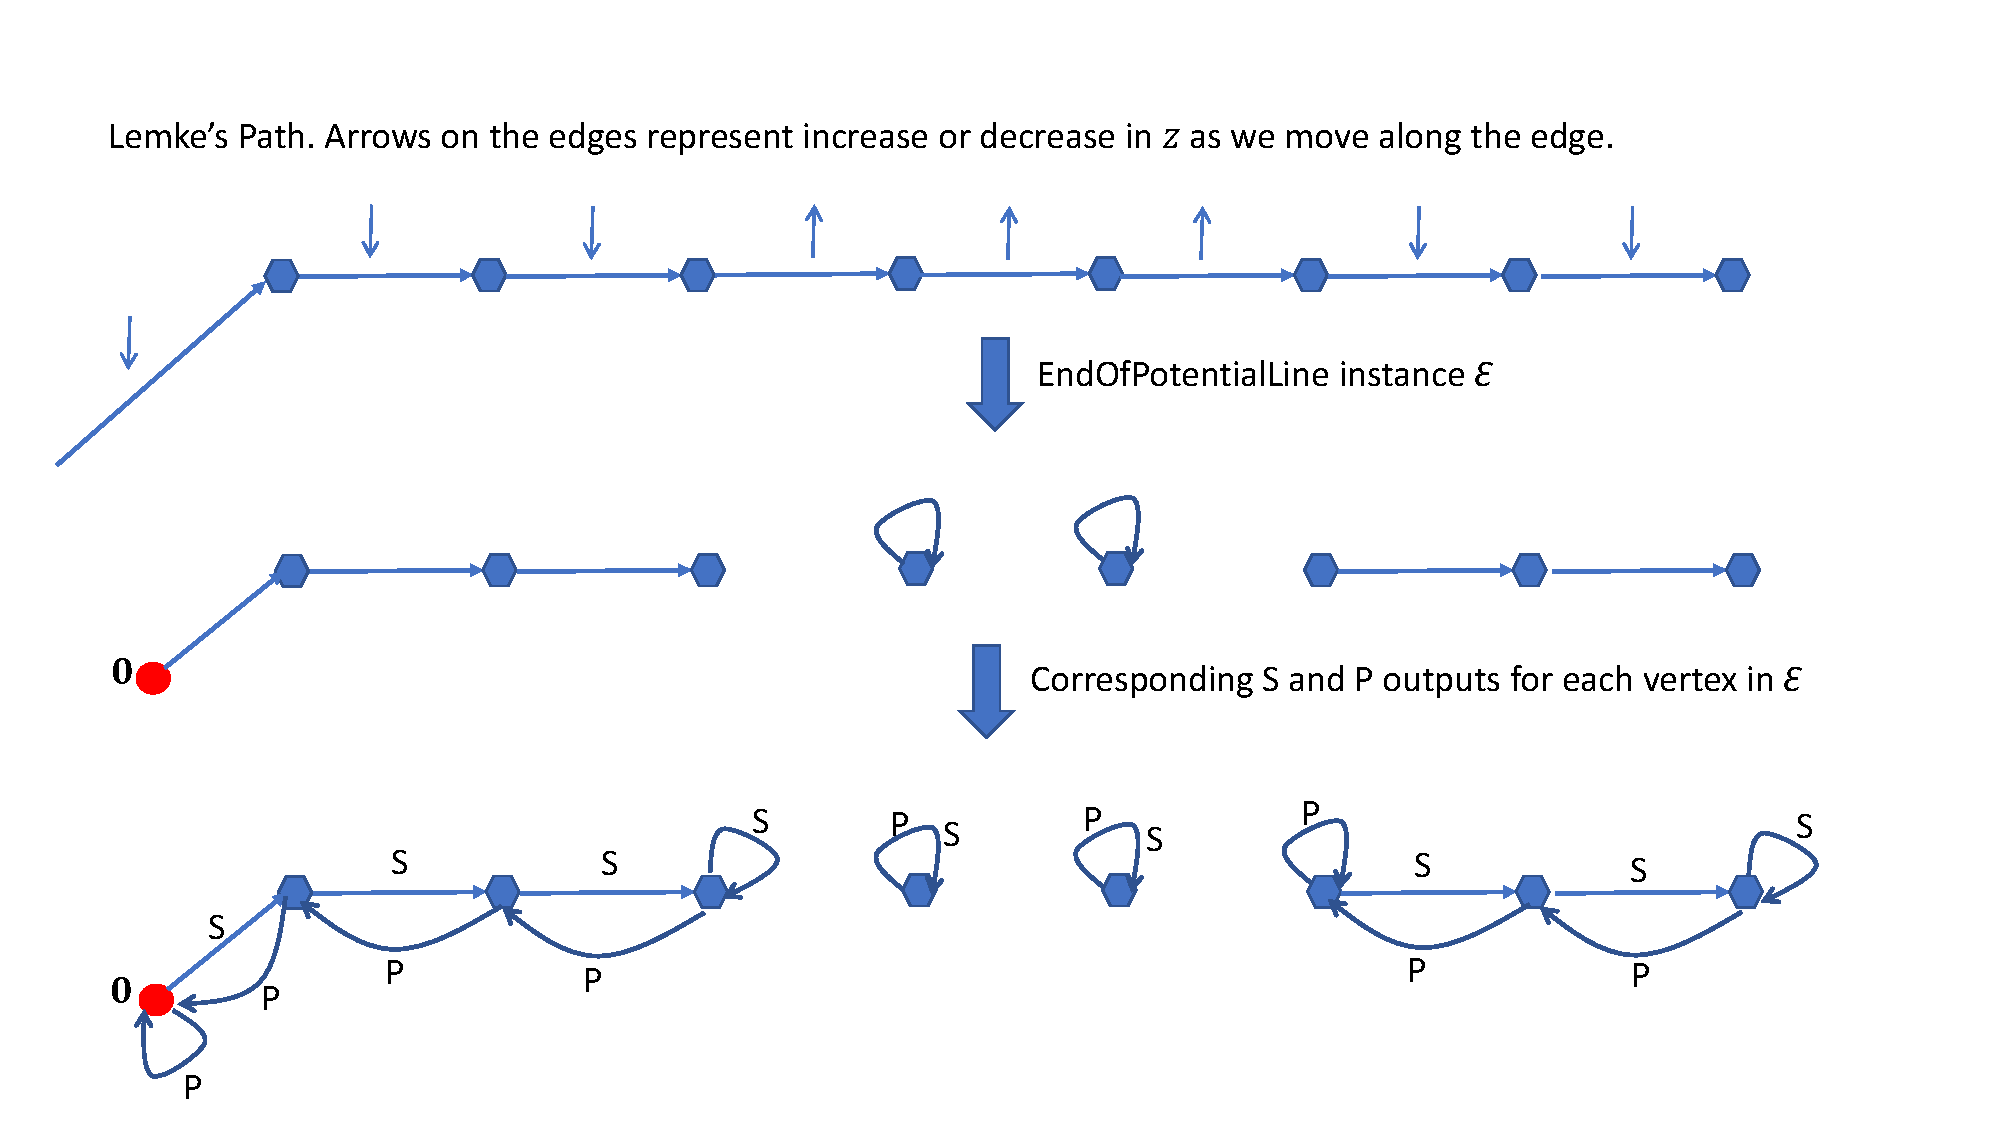
\includegraphics[width=\textwidth]{plcp-fig.pdf}
 \caption{Construction of $S$ and $P$ for \EOPL instance $\CE$ from the Lemke
 	path. The first path is the Lemke path and the arrows on its edges indicate
 	whether the value of $z$ increases or decreases along the edge.  Note that
 	the end or start of a path in $\CE$, which is an intermediate vertex in
 	Lemke path that has either decreased and then increased, or increased and then
 	decreased in the value of $z$, is a violation of $M$ being a $P$ matrix
 	\cite{cottle2009linear}, i.e., $\PLt$ type solution of
 	\PLCP.}
 	\label{fig:path}
\end{figure}   


The main idea behind procedures $S$ and $P$, given in Tables \ref{tab:S} and
\ref{tab:P} respectively, is the following (also see Figure \ref{fig:path}):
Make dummy configurations in $\vert$ point to themselves with cycles of
length one, so that they can never be solutions. 
The starting vertex $0^n \in \vert$ points to the configuration that corresponds
to the first vertex of the Lemke path, namely $\uu^0=\ite(\yy^0,\ps^0,z^0)$. 
Precisely, $S(0^n)=\uu^0$, $P(\uu^0)=0^n$ and $P(0^n)=0^n$ (start of
a path). 

For the remaining cases, let $\uu\in \vert$ have corresponding representation
$\xx=(\yy,\ps,z)\in \CPol$, and suppose $\xx$ has a duplicate label. As one
traverses a Lemke path for a P-LCPs, the value of $z$ monotonically decreases.
So, for $S(\uu)$ we compute the adjacent vertex $\xx'=(\yy',\ps',z')$ of $\xx$
on Lemke path such that the edge goes from $\xx$ to $\xx'$, and if the $z'<z$,
as expected, then we point $S(\uu)$ to configuration of $\xx'$ namely
$\ite(\xx')$. Otherwise, we let $S(\uu)=\uu$. Similarly, for $P(\uu)$, we find
$\xx'$ such that edge is from $\xx'$ to $\xx$, and then we let $P(\uu)$ be
$\ite(\xx')$ if $z'>z$ as expected, otherwise $P(\uu)=\uu$. 

For the case when $\xx$ does not have a duplicate label, then we have $z=0$. This is
handled separately since such a vertex has exactly one incident edge on the Lemke
path, namely the one obtained by relaxing $z=0$. According to the direction of 
this edge, we do similar process as before. For example, if the edge goes from 
$\xx$ to $\xx'$, then, if $z'<z$, we set $S(\uu)=\ite(\xx')$ else $S(\uu)=\uu$,
and we always set $P(\uu)=\uu$.  In case the edge goes from $\xx'$ to $\xx$, we
always set $S(\uu)=\uu$, and we set $P(\uu)$ depending on whether or not $z'>z$.

%If $\xx$ is a solution of the original LCP, i.e., $z=0$, then exactly one of $S(\uu)$ or $P(\uu)$ would point to the configuration of the vertex obtained by relaxing $z=0$ at $xx$, while the other will point back to $\uu$ itself. Which one of the two cases happen depends on what orientation corresponding edge on Lemke's path has. 
%
%For the rest, if $l$ is the duplicate label at $\xx$ then let $\xx^1$ and $\xx^2$ be the two vertices obtained by relaxing $y_l=0$ and $s_l=0$ at $\xx$. Lemke's algoithm must have traversed either $\xx^1$ to $\xx$ to $\xx^2$, or $\xx^2$ to $\xx$ to $\xx^1$. Which of the two would tell us output of $S(\uu)$ and $P(\uu)$. Todd \cite{} gives a polynomial time procedure to find out which one is the case based on signs of certain determinants of matrices formed using the sets of non-zero and zero variables at these three vertices, and $(M,\qq)$. Based on this we output either representation of $\xx^1$ or $\xx^2$. 
\medskip

The potential function $\pot$, formally defined in Table \ref{tab:F},
gives a value of zero to dummy vertices and the starting vertex $0^n$. To all
other vertices, essentially it is $((z^0-z) * \Delta^2)+1$. Since value of $z$
starts at $z^0$ and keeps decreasing on the Lemke path this value will keep
increasing starting from zero at the starting vertex $0^n$. Multiplication by
$\Delta^2$ will ensure that if $z_1>z_2$ then the corresponding potential values 
will differ by at least one. This is because, since $z_1$ and $z_2$ are 
coordinates of two vertices of polytope $\CPol$, their maximum value is $\Delta$
and their denominator is also bounded above by $\Delta$. Hence $z_1-z_2\le
1/\Delta^2$ (Lemma \ref{lem:pot}).  
% REWRITE
%Thus, if after change of scales $1/2*\Delta^2$ defines a unit then
%corresponding integers will differ by at least one. 

To show correctness of the reduction we need to show two things: $(i)$ All the procedures are well-defined and polynomial time. $(ii)$ We can construct a solution of $\CI$ from a solution of $\CE$ in polynomial time. 



\begin{table}
\begin{minipage}{0.73\textwidth}
\caption{Successor Procedure $S(\uu)$}\label{tab:S}
\begin{tabular}{|l|}
\hline
%$S(\uu)$\\
%\small{
\hspace{0pt}{\bf If} $\isvalid(\uu)=0$ {\bf then} {\bf Return} $\uu$\\
\hspace{0pt}{\bf If} $\uu=0^n$ {\bf then} {\bf Return} $\ite(\yy^0,\ps^0,z^0)$\\
\hspace{0pt}$\xx=(\yy,\ps,z) \leftarrow \eti(\uu)$\\
%\hspace{5pt} {\bf If} $z=0$ {\bf then} {\bf Return} $\uu$
\hspace{0pt}{\bf If} $z=0$ {\bf then} \\
\hspace{5pt} $\xx^1\leftarrow$ vertex obtained by relaxing $z=0$ at $\xx$ in $\CPol$. \\
\hspace{5pt} {\bf If} Todd \cite{todd1976orientation} prescribes edge from $\xx$ to $\xx^1$ \\
\hspace{10pt} {\bf then} set $\xx'\leftarrow \xx^1$. {\bf Else Return} $\uu$ \\
\hspace{0pt}{\bf Else} set $l\leftarrow $ duplicate label at $\xx$\\
%\hspace{5pt} $(\yy',\ps',z') \leftarrow$ Next vertex from $(\yy,\ps,z)$ in $\CPol$ as preѕcribed by Todd \cite{todd}. 
\hspace{5pt} $\xx^1\leftarrow $ vertex obtained by relaxing $y_l=0$ at $\xx$ in $\CPol$ \\
\hspace{5pt} $\xx^2\leftarrow $ vertex obtained by relaxing $s_l=0$ at $\xx$ in $\CPol$ \\
\hspace{5pt} {\bf If} Todd \cite{todd1976orientation} prescribes edge from $\xx$ to $\xx^1$ \\
\hspace{10pt} {\bf then} $\xx'=\xx^1$ \\
\hspace{5pt} {\bf Else} $\xx'=\xx^2$\\
\hspace{0pt}Let $\xx'$ be $(\yy',\ps',z')$. \\
\hspace{0pt}{\bf If} $z>z'$ {\bf then} {\bf Return} $\ite(\xx')$. {\bf Else} {\bf Return} $\uu$.\\
%\hspace{5pt} {\bf Return} $\ite(\xx')$.
%}
\hline
\end{tabular}
\end{minipage}%
\hspace{-1cm}
\begin{minipage}{0.23\textwidth}
\caption{Potential Value $\pot(\uu)$}\label{tab:F}
\begin{tabular}{|l|}
\hline
%\small{
%$\pot(\uu)$\\
\hspace{0pt} {\bf If} $\isvalid(\uu)=0$ \\
\hspace{5pt} {\bf then} {\bf Return} $0$\\
\hspace{0pt} {\bf If} $\uu=0^n$\\
\hspace{5pt}  {\bf then} {\bf Return} $0$\\
\hspace{0pt} $(\yy,\ps,z) \leftarrow \eti(\uu)$\\
\hspace{0pt} {\bf Return} $\lfloor \Delta^2*(\Delta -z)\rfloor$\\
%}
\hline
\end{tabular}
\end{minipage}
\end{table}



\begin{table}[!htb]
\caption{Predecessor Procedure $P(\uu)$}\label{tab:P}
\begin{tabular}{|l|}
\hline
%$P(\uu)$\\
%\small{
\hspace{0pt} {\bf If} $\isvalid(\uu)=0$ {\bf then} {\bf Return} $\uu$\\
\hspace{0pt} {\bf If} $\uu=0^n$ {\bf then} {\bf Return} $\uu$\\
\hspace{0pt} $(\yy,\ps,z) \leftarrow \eti(\uu)$\\
\hspace{0pt} {\bf If} $(\yy,\ps,z)=(\yy^0,\ps^0,z^0)$ {\bf then} {\bf Return} $0^n$\\
%\hspace{5pt} $l\leftarrow $ duplicate label at $(\yy,\ps,z)$, $(\yy',\ps',z') \leftarrow $ $Prev(\vv,l)$.\\
%\hspace{5pt} $(\yy',\ps',z') \leftarrow$ Previous vertex from $(\yy,\ps,z)$ in $\CPol$ as preѕcribed by Todd \cite{todd}. \\
\hspace{0pt} {\bf If} $z=0$ {\bf then} \\
\hspace{5pt} $\xx^1\leftarrow$ vertex obtained by relaxing $z=0$ at $\xx$ in $\CPol$. \\
\hspace{5pt} {\bf If} Todd \cite{todd1976orientation} prescribes edge from $\xx^1$ to $\xx$ {\bf then} set $\xx'\leftarrow \xx^1$. {\bf Else Return} $\uu$\\
\hspace{0pt} {\bf Else}\\
\hspace{5pt} $l\leftarrow $ duplicate label at $\xx$\\
\hspace{5pt} $\xx^1\leftarrow $ vertex obtained by relaxing $y_l=0$ at $\xx$ in $\CPol$ \\
\hspace{5pt} $\xx^2\leftarrow $ vertex obtained by relaxing $s_l=0$ at $\xx$ in $\CPol$ \\
\hspace{5pt} {\bf If} Todd \cite{todd1976orientation} prescribes edge from $\xx^1$ to $\xx$ {\bf then} $\xx'=\xx^1$ {\bf Else} $\xx'=\xx^2$\\
\hspace{0pt} Let $\xx'$ be $(\yy',\ps',z')$. {\bf If} $z<z'$ {\bf then} {\bf Return} $\ite(\xx')$. {\bf Else} {\bf Return} $\uu$.\\
%\hspace{5pt} {\bf Return} $\ite(\xx')$.
%}
\hline
\end{tabular}
\end{table}



\begin{lemma}\label{lem:PSF}
Functions $P$, $S$ and $\pot$ of instance $\CE$ are well defined, making $\CE$ a valid \EOPL instance. 
\end{lemma}
%\begin{proof}
%Since all the three procedures are polynomial time in $\CL$, they can be defined
%	by $poly(\CL)$ sized Boolean circuits. Furthermore, for any $\uu \in \vert$,
%	$S(\uu),P(\uu) \in \vert$. For $\pot$, since value of $z \in [0,\ \Delta-1]$ we
%	have $0\le \Delta^2(\Delta-z)\le \Delta^3$. Therefore, $\pot(\uu)$ is an
%	integer that is at most $2*\Delta^3$ and hence is in set $\{0,\dots, 2^m-1\}$. 
%\end{proof}

There are two possible types of solutions of an \EOPL instance. One indicates
the beginning or end of a line, and the other is a vertex with locally optimal
potential (that does not point to itself). 
First we show that the latter case never arise. For this, we need the
next lemma, which shows that potential differences in two adjacent
configurations adheres to differences in the value of $z$ at corresponding
vertices.

\begin{lemma}\label{lem:pot}
Let $\uu \neq \uu'$ be two valid configurations, i.e.,
	$\isvalid(\uu)=\isvalid(\uu')=1$, and let $(\yy,\ps,z)$ and $(\yy',\ps',z')$
	be the corresponding vertices in $\CPol$. Then the following holds: $(i)$
	$\pot(\uu)=\pot(\uu')$ iff $z=z'$. $(ii)$ $\pot(\uu)>\pot(\uu')$ iff $z<z'$.
\end{lemma}
%\begin{proof}
%Among the valid configurations all except $0^n$ has positive $\pot$ value. Therefore, wlog let $\uu,\uu'\neq 0^n$. For these we have $\pot(\uu)=\lfloor \Delta^2*(\Delta -z)\rfloor$, and $\pot(\uu')=\lfloor \Delta^2*(\Delta -z')\rfloor$. 
%
%Note that since both $z$ and $z'$ are coordinates of vertices of $\CPol$, whose description has highest coefficient of $\max\{\max_{i,j\in [d]} M(i,j),\max_{i\in [d]} |q_i|\}$, and therefore their numerator and denominator both are bounded above by $\Delta$. Therefore, if $z< z'$ then 
%\[
%z'-z\ge \frac{1}{\Delta^2} \Rightarrow ((\Delta-z) - (\Delta - z'))*\Delta^2 \ge 1 \Rightarrow \pot(\uu)-\pot(\uu') \ge 1
%\]
%
%For $(i)$, if $z=z'$ then clearly $\pot(\uu)=\pot(\uu')$, and from the above argument it also follows that if $\pot(\uu)= \pot(\uu')$ then it can not be the case that $z\neq z'$. Similarly for $(ii)$, if $\pot(\uu)>\pot(\uu')$ then clearly, $z'>z$, and from the above argument it follows that if $z'>z$ then it can not be the case that $\pot(\uu')\ge \pot(\uu)$. 
%\end{proof}

Using the above lemma, we will next show that instance $\CE$ has no local maximizer. 

\begin{lemma}\label{lem:t}
Let $\uu,\vv \in \vert$ s.t. $\uu\neq \vv$, $\vv=S(\uu)$, and $\uu=P(\vv)$. Then $\pot(\uu)< \pot(\vv)$.
\end{lemma}
\begin{proof}
Let $\xx=(\yy,\ps,z)$ and $\xx'=(\yy',\ps',z')$ be the vertices in polyhedron $\CPol$ corresponding to $\uu$ and $\vv$ respectively. From the construction of $\vv=S(\uu)$ implies that $z'<z$. Therefore, using Lemma \ref{lem:pot} it follows that $\pot(\vv)<\pot(\uu)$.
%Both $\uu$ and $\vv$ can not be dummy configurations because otherwise they will point to themselves in $P$ and $S$ both. For the rest let $\xx=(\yy,\ps,z)$ and $\xx'=(\yy',\ps',z')$ be the vertices in polyhedron $\CPol$ corresponding to $\uu$ and $\vv$ respectively. Since these are not dummy, we have an edge from $\xx$ to $\xx'$. Further, using Lemma \ref{lem:pot} it must be the case that $z<z'$. In otherwords, if $\sigma=\xx'-\xx$ then $\simga(z)>0$. This contradicts $M$ being a P-matrix, and the submatrix corresponding non-zero gives a witness. 
\end{proof}

Due to Lemma \ref{lem:t} the only type of solutions available in $\CE$ is where $S(P(\uu))\neq \uu$ and $P(S(\uu))\neq \uu$. Next two lemmas shows how to construct solutions of $\CI$ from these. 

\begin{lemma}\label{lem:t1}
Let $\uu \in \vert$, $\uu \neq 0^n$. % be such that $\isvalid(\uu)=1$, and let $(\yy,\ps,z)=\eti(\uu)$. 
If $P(S(\uu))\neq \uu$ or $S(P(\uu))\neq \uu$, then $\isvalid(\uu)=1$, and for $(\yy,\ps,z)=\eti(\uu)$ if $z=0$ then $\yy$ is a $\PLo$ type solution of \PLCP instance $\CI=(M,\qq)$. 
\end{lemma}
\begin{proof}
By construction, if $\isvalid(\uu) = 0$, then $S(P(\uu))=\uu$ and $P(S(\uu))=\uu$, therefore $\isvalid(\uu)=0$ when $\uu$ has a predecessor or successor different from $\uu$.
Given this, from Lemma \ref{lem:vert} we know that $(\yy,\ps,z)$ is a feasible vertex in (\ref{eq:c}). Therefore, if $z=0$ then using Lemma \ref{lem:lemke1} we have a solution of the LCP (\ref{eq:lcp}), {\em i.e.,} a type $\PLo$ solution of our \PLCP instance $\CI=(\MM,\qq)$.
%
%If it has a duplicate label, then it has two incident edges say from vertices $\xx'$ and $\xx''$. Let the corresponding configurations in $\CE$ be $\uu'$ and $\uu''$ respectively. Due to Lemma \ref{lem:vert}, we can consistently go between $\uu$'s and $\xx$'s using $\ite$ and $\eti$ procedues. Further, if $\uu'=S(\uu)$ then when we apply $P$ to $\uu'$ we will get back $\uu$, due to the property of Lemke's algorithm and cannonical orientation obtained by Todd \cite{todd}. Similarly, if $\uu''=P(\uu)$ then $S(\uu'')$ will give $\uu$ back. Therefore, $\uu$ can not be a vertex with duplicate label.
%
%The only remaining valid configurations correspond to vertices of $\CPol$ that satisfy $y_is_i=0,\ \forall i \in[d]$, and $z=0$. Since solutions of (\ref{eq:c}) are exactly the solutions of (\ref{eq:lcp}) (Lemma \ref{lem:lemke1}) we get $\PLo$ type solution of our given PLCP instance $\CI=(M,\qq)$.
\end{proof}

\begin{lemma}\label{lem:t2}
Let $\uu \in \vert$, $\uu \neq 0^n$ such that $P(S(\uu))\neq \uu$ or $S(P(\uu))\neq \uu$, and let $\xx=(\yy,\ps,z)=\eti(\uu)$. 
If $z\neq 0$ then $\xx$ has a duplicate label, say $l$. And for directions $\sigma_1$ and $\sigma_2$ obtained by relaxing $y_l=0$ and $s_l=0$ respectively at $\xx$, we have $\sigma_1(z)*\sigma_2(z)\ge 0$, where $\sigma_i(z)$ is the coordinate corresponding to $z$. 
\end{lemma}
\begin{proof}
From Lemma \ref{lem:t1} we know that $\isvalid(\uu)=1$, and therefore from Lemma \ref{lem:vert}, $\xx$ is a feasible vertex in (\ref{eq:c}).
From the last line of Tables \ref{tab:S} and \ref{tab:P} observe that $S(\uu)$ points to the configuration of vertex next to $\xx$ on Lemke's path only if it has lower $z$ value otherwise it gives back $\uu$, and similarly $P(\uu)$ points to the previous only if value of $z$ increases.

%For both the cases we have that either $S(\uu)\neq \uu$ or $P(\uu)\neq \uu$. 
%}

First consider the case when $P(S(\uu))\neq \uu$. Let $\vv=S(\uu)$ and corresponding vertex in $\CPol$ be $(\yy',\ps',z')=\eti(\vv)$. 
If $\vv\neq \uu$, then from the above observation we know that $z'>z$, and in that
case again by construction of $P$ we will have $P(\vv)=\uu$, contradicting
$P(S(\uu))\neq \uu$. Therefore, it must be the case that $\vv=\uu$.
Since $z\neq 0$ this happens only when the next vertex on Lemke path after $\xx$ has
higher value of $z$ (by above observation). As a consequence of $\vv=\uu$, we also have $P(\uu)\neq \uu$. By construction of $P$ this implies for 
$(\yy'',\ps'',z'')=\eti(P(\uu))$, $z''>z$. Putting both together we get 
increase in $z$ when we relax $y_l=0$ as well as when we relax $s_l=0$ at
$\xx$.

For the second case $S(P(\uu))\neq \uu$ similar argument gives that value of $z$ decreases when we relax $y_l=0$ as well as when we relax $s_l=0$ at
$\xx$. The proof follows.
\end{proof}

Finally, we are ready to prove our main result of this section using Lemmas
\ref{lem:t}, \ref{lem:t1} and \ref{lem:t2}. Together with Lemma \ref{lem:t2},
we will use the fact that on Lemke path $z$ monotonically decreases if $M$ is a
P-matrix or else we get a witness that $M$ is not a
P-matrix~\cite{cottle2009linear}. 
%Lemmas \ref{lem:t1} and \ref{lem:t2} gives the two possible types of solutions
%of the PLCP problem. That is either actual solution of the corresponding LCP
%instance, or a witness that the given matrix is not a $P$-matrix. Recall that
%checking the latter is co-NP-complete. Thus next theorem follows from Lemmas
%\ref{lem:PSF}, \ref{lem:t1} and \ref{lem:t2}.

\begin{theorem}
\PLCP reduces to \EOPL in polynomial-time. 
\end{theorem}
\begin{proof}
	Given an instance of $\CI=(\MM,\qq)$ of \PLCP, where $M\in \Real^{d\times d}$ and $\qq\in \Real^{d\times 1}$ reduce it to an instance $\CE$ of \EOPL as described above with vertex set $\vert=\{0,1\}^{2d}$ and procedures $S$, $P$ and $\pot$ as given in Table \ref{tab:S}, \ref{tab:P}, and \ref{tab:F} respectively.

Among solutions of \EOPL instance $\CE$, there is no local potential maximizer,
	i.e., $\uu\neq \vv$ such that $\vv=S(\uu)$, $\uu=P(\vv)$ and $\pot(\uu)>\pot(\vv)$
	due to Lemma \ref{lem:t}. We get a solution $\uu \neq 0$ such that either
	$S(P(\uu))\neq \uu$ or $P(S(\uu))\neq \uu$, then by Lemma \ref{lem:t1} it is
	valid configuration and has a corresponding vertex $\xx=(\yy,\ps,z)$ in
	$\CPol$. Again by Lemma~\ref{lem:t1} if $z=0$ then $\yy$ is a $\PLo$ type solution
	of our \PLCP instance $\CI$. On the other hand, if $z>0$ then from Lemma
	\ref{lem:t2} we get that on both the two adjacent edges to $\xx$ on Lemke
	path the value of $z$ either increases or deceases. This gives us a minor of $M$
	which is non-positive~\cite{cottle2009linear}, 
	i.e., a $\PLt$ type solution of the $\PLCP$	instance $\CI$.
\end{proof}

\newpage

\section{Missing Procedures and Proofs from Section~\ref{sec:PLCPtoEOPL}}\label{app:PLCPtoEOPL}
\subsection{Procedures $\isvalid$, $\ite$, and $\eti$}\label{app:proc}
\begin{table}[!hbt]
\caption{Procedure \isvalid(\uu)}\label{tab:iv}
\begin{tabular}{|l|}
\hline
\hspace{5pt} {\bf If} $\uu=0^{n}$ {\bf then} {\bf Return} 1\\
\hspace{5pt} {\bf Else} let $\tau = (u_{(d+1)}+\dots+u_{2d})$\\
\hspace{15pt} {\bf If} $\tau> 1$ {\bf then} {\bf Return} 0\\
\hspace{15pt} Let $S\leftarrow \emptyset$. \% set of tight inequalities. \\
\hspace{15pt} {\bf If} $\tau = 0$ {\bf then} $S=S\cup \{ z=0\}$. \\
\hspace{15pt} {\bf Else}\\
\hspace{30pt} Set $l\leftarrow $ index of the non-zero coordinate in vector $(u_{(d+1)},\dots,u_{2d})$. \\
\hspace{30pt} Set $S=\{y_l=0, s_l=0\}$.\\
%Set $\yy\leftarrow \zeros, \ps\leftarrow zeros, z\leftarrow 0$. \\
\hspace{15pt} {\bf For} each $i$ from $1$ to $d$ {\bf do} \\
\hspace{30pt} {\bf If} $u_i=0$ {\bf then} $S=S\cup \{y_i=0\}$, {\bf Else} $S=S\cup \{s_i=0\}$\\
\hspace{15pt} Let $A$ be a matrix formed by lhs of equalities $M\yy+\ps -\ones z=\qq$ and that of set $S$\\
\hspace{15pt} Let $\bb$ be the corresponding rhs, namely $\bb=[\qq; \zeros_{d\times 1}]$.\\
\hspace{15pt} Let $(\yy',\ps',z') \leftarrow \bb * A^{-1}$\\
\hspace{15pt} {\bf If} $(\yy',\ps',z') \in \CPol$ {\bf then} {\bf Return} 1, {\bf Else} {\bf Return} 0 \\
\hline
\end{tabular}
\end{table}

\begin{table}[!hbt]
\caption{Procedures \ite(\uu) and \eti(\yy,\ps,z)}\label{tab:ei}
\begin{tabular}{|l|}
\hline
\begin{tabular}{l}
$\ite(\yy,\ps,z)$ \\ \hline
\hspace{5pt} {\bf If} $\exists i \in [d]$ s.t. $y_i * s_i \neq 0$ {\bf then} {\bf Return} $(\zeros_{(2d-2)\times 1};1;1)$ \% Invalid \\
\hspace{5pt} Set $\uu\leftarrow \zeros_{2d\times 1}$. Let $DL=\{i\in [d]\ |\ y_i=0\mbox{ and } s_i=0\}$.\\
\hspace{5pt} {\bf If} $|DL|>1$ {\bf then} {\bf Return} $(\zeros_{(2d-2)\times 1};1;1)$ \%In valid \\
\hspace{5pt} {\bf If} $|DL|=1$ {\bf then} for $i\in DL$, set $u_i\leftarrow 1$\\
\hspace{5pt} {\bf For} each $i\in [d]$ {\bf If} $s_i=0$ {\bf then} set $u_{d+i}\leftarrow 1$\\
\hspace{5pt} {\bf Return} $\uu$
\end{tabular}
\\ \hline
\begin{tabular}{l}
$\eti(\uu)$  \\ \hline
\hspace{5pt} {\bf If} $\uu=0^n$ {\bf then} {\bf Return} $(\zeros_{d \times 1}, \qq+z^0+1, z^0+1)$ \% This case will never happen\\
\hspace{5pt} {\bf If} \isvalid(\uu)=0 {\bf then} {\bf Return} $\zeros_{(2d+1) \times 1}$\\
\hspace{5pt} Let $\tau = (u_{(d+1)}+\dots+u_{2d})$\\
\hspace{5pt} Let $S\leftarrow \emptyset$. \% set of tight inequalities. \\
\hspace{5pt} {\bf If} $\tau = 0$ {\bf then} $S=S\cup \{ z=0\}$. \\
\hspace{5pt} {\bf Else}\\
\hspace{15pt} Set $l\leftarrow $ index of non-zero coordinate in vector $(u_{(d+1)},\dots,u_{2d})$. \\
\hspace{15pt} Set $S=\{y_l=0, s_l=0\}$.\\
%Set $\yy\leftarrow \zeros, \ps\leftarrow zeros, z\leftarrow 0$. \\
\hspace{5pt} {\bf For} each $i$ from $1$ to $d$ {\bf do} \\
\hspace{15pt} {\bf If} $u_i=0$ {\bf then} $S=S\cup \{y_i=0\}$, {\bf Else} $S=S\cup \{s_i=0\}$\\
\hspace{5pt} Let $A$ be a matrix formed by lhs of equalities $M\yy+\ps -\ones z=\qq$ and that of set $S$\\
\hspace{5pt} Let $\bb$ be the corresponding rhs, namely $\bb=[\qq; \zeros_{d\times 1}]$.\\
\hspace{5pt} {\bf Return} $\bb * A^{-1}$\\
\end{tabular}\\
\hline
\end{tabular}
\end{table}

\subsection{Proof of Lemma~\ref{lem:vert}}

\textbf{Lemma \ref{lem:vert}} (restated) : \emph{
If $\isvalid(\uu)=1$ then $\uu=\ite(\eti(\uu))$, and the corresponding vertex $(\yy,\ps,z)\in \eti(\uu)$ of $\CPol$ is feasible in (\ref{eq:c}). If $(\yy,\ps,z)$ is a feasible vertex of (\ref{eq:c}) then $\uu=\ite(\yy,\ps,z)$ is a valid configuration, {\em i.e.,} $\isvalid(\uu)=1$.
}
\begin{proof}
The only thing that can go wrong is that the matrix $A$ generated in $\isvalid$ and $\eti$ procedures are singular, or the set of double labels $DL$ generated in $\ite$ has more than one elements. 
Each of these are possible only when more than $2d+1$ equalities of $\CPol$ hold at the corresponding point $(\yy,\ps,z)$, violating non-degeneracy assumption. 
\end{proof}

\subsection{Proof of Lemma~\ref{lem:PSF}}

\textbf{Lemma \ref{lem:PSF}} (restated) : \emph{
Functions $P$, $S$ and $\pot$ of instance $\CE$ are well defined, making $\CE$ a valid \EOPL instance. 
}
\begin{proof}
Since all three procedures are polynomial-time in $\CL$, they can be defined
by $poly(\CL)$-sized Boolean circuits. Furthermore, for any $\uu \in \vert$,
we have that $S(\uu),P(\uu) \in \vert$. For~$\pot$, 
since the value of $z \in [0,\ \Delta-1]$, we
have $0\le \Delta^2(\Delta-z)\le \Delta^3$. Therefore, $\pot(\uu)$ is an
integer that is at most $2 \cdot \Delta^3$ and hence is in set $\{0,\dots, 2^m-1\}$. 
\end{proof}

\subsection{Proof of Lemma~\ref{lem:pot}}

\textbf{Lemma \ref{lem:pot}} (restated) : \emph{
Let $\uu \neq \uu'$ be two valid configurations, i.e.,
	$\isvalid(\uu)=\isvalid(\uu')=1$, and let $(\yy,\ps,z)$ and $(\yy',\ps',z')$
	be the corresponding vertices in $\CPol$. Then the following holds: $(i)$
	$\pot(\uu)=\pot(\uu')$ iff $z=z'$. $(ii)$ $\pot(\uu)>\pot(\uu')$ iff $z<z'$.
}
\begin{proof}
Among the valid configurations all except $\zeros$ has positive $\pot$ value. Therefore, wlog let $\uu,\uu'\neq \zeros$. For these we have $\pot(\uu)=\lfloor \Delta^2*(\Delta -z)\rfloor$, and $\pot(\uu')=\lfloor \Delta^2*(\Delta -z')\rfloor$. 

Note that since both $z$ and $z'$ are coordinates of vertices of $\CPol$, whose description has highest coefficient of $\max\{\max_{i,j\in [d]} M(i,j),\max_{i\in [d]} |q_i|\}$, and therefore their numerator and denominator both are bounded above by $\Delta$. Therefore, if $z< z'$ then we have 
\[
z'-z\ge \frac{1}{\Delta^2} \Rightarrow ((\Delta-z) - (\Delta - z'))*\Delta^2 \ge 1 \Rightarrow \pot(\uu)-\pot(\uu') \ge 1.
\]

For $(i)$, if $z=z'$ then clearly $\pot(\uu)=\pot(\uu')$, and from the above argument it also follows that if $\pot(\uu)= \pot(\uu')$ then it can not be the case that $z\neq z'$. Similarly for $(ii)$, if $\pot(\uu)>\pot(\uu')$ then clearly, $z'>z$, and from the above argument it follows that if $z'>z$ then it can not be the case that $\pot(\uu')\ge \pot(\uu)$. 
\end{proof}

\section{Pseudo-code for Lemke's algorithm}
\label{app:lemke}

%\begin{table}[!htb]
%\caption{Lemke's Complementary Pivot Algorithm}\label{tab:lemke}
\begin{tabular}{|l|}
\hline
\hspace{5pt} {\bf If} $\qq\ge 0$ {\bf then} {\bf Return} $\yy\leftarrow \zeros$ \\
\hspace{5pt} $\yy\leftarrow 0, z\leftarrow |\min_{i \in [d]} q_i|, \ps=\qq+z\ones$\\
\hspace{5pt} $i\leftarrow $ duplicate label at vertex $(\yy,\ps,z)$ in $\CPol$. $flag\leftarrow 1$ \\
\hspace{5pt} {\bf While} $z>0$ {\bf do}\\
\hspace{10pt} {\bf If} $flag=1$ {\bf then} set $(\yy',\ps',z')\leftarrow $ vertex obtained by relaxing $y_i=0$ at $(\yy,\ps,z)$ in $\CPol$\\
\hspace{10pt} {\bf Else} set $(\yy',\ps',z')\leftarrow $ vertex obtained by relaxing $s_i=0$ at $(\yy,\ps,z)$ in $\CPol$\\
\hspace{10pt} {\bf If} $z>0$ {\bf then}\\
\hspace{15pt} $i \leftarrow $ duplicate label at $(\yy',\ps',z')$\\
\hspace{15pt} {\bf If} $v_i>0$ and $v'_i=0$ {\bf then} $flag\leftarrow 1$. {\bf Else} $flag\leftarrow 0$\\
\hspace{15pt} $(\yy,\ps,z)\leftarrow(\yy',\ps',z')$\\
\hspace{5pt} End {\bf While} \\
\hspace{5pt} {\bf Return} $\yy$\\
\hline
\end{tabular}
%\end{table}

\chapter{\TwoDContractionMap to \EOPL}
\label{sec:twoDContractionMapToEOPL}
In this chapter, we reduce a slightly weaker variant of \CM to \EOPL. Aside from providing further evidence for the \CLS-hardness of \EOPL, the technique we introduce in this reduction is of independent interest and we believe may be applicable to reducing \CM, \MMCM, or \MBanach to \EOPL, which would show \CLS-completeness of \EOPL in the latter two cases.

We restate the definition of \EOPL here for convenience:

\begin{definition}[\EOPL]
\label{def:EOPL2}
Given Boolean circuits $S,P : \Set{0,1}^n \to \Set{0,1}^n$ such that $P(0^n) =0^n\neq S(0^n)$ and a Boolean circuit $V: \Set{0,1}^n \to \Set{0,1,\dotsc,2^m - 1}$ such that $V(0^n) = 0$ find one of the following:
\begin{enumerate}[label=(R\arabic*)]
\item A point $x \in \Set{0,1}^n$ such that $S(P(x)) \neq x \neq 0^n$ or $P(S(x)) \neq x$. \label{eopl2:eol}
\item A point $x \in \Set{0,1}^n$ such that $x \neq S(x)$, $P(S(x)) = x$, and $V(S(x)) - V(x) \leq 0$. \label{eopl2:bad_potential}
\end{enumerate}
\end{definition}


The variant of \CM (Definition~\ref{def:contractionmap}) we will consider here differs from \CM in that the domain and range of the map is $[0,1]^2$ instead of $[0,1]^3$, and in that the norm under consideration is required to be a $p$-norm.
\begin{definition}[\TwoDContractionMap] 
  \label{def:2DContractionMap}
We are given as input an arithmetic circuit computing $f: [0,1]^2\to [0,1]^2$,
a choice of $p$-norm $\Norm{\cdot}_p$, constants \mbox{$c \in (0,1)$}
and $\delta > 0$. It is asserted that $f$ is $c$-contracting with respect to $\Norm{\cdot}_p$.
The goal is to find
\begin{enumerate}[label=(E\arabic*)]
\item a point $x\in [0,1]^2$ such that $\Norm{f(x),x}_p \leq \delta$, \label{2dcm:fixpoint}
\item or two points $x,y\in [0,1]^3$ such that $\Norm{f(x) - f(y)}_p/\Norm{x-y}_p > c$. \label{2dcm:violation}
\end{enumerate}
\end{definition}

The observation underlying the reduction is that applying the standard reduction from the computational version of Brouwer's Fixed-Point Theorem to Sperner's Lemma in the special case of contraction maps results in instances of Sperner's Lemma in which the the given Sperner path has a very special structure. This structure then allows us to assign a consistent potential function to the vertices of the \PPAD graph created in the reduction from Sperner's Lemma to \EOL.

The precise version of the Sperner problem we will use is the following, due to Papadimitriou \cite{papadimitriou1994complexity}:
\begin{definition}[\Sperner] 
  \label{def:Sperner}
  We are given as input an algorithm
  \[\mycolor: \Set{0/n,1/n,\dotsc,n/n}^2 \to \Set{\Blue, \Red, \Yellow}\] that computes a color for the vertices of an $n\times n$ subdivision of the unit square in polynomial-time (in the binary representation of $n$). The coloring given by the algorithm satisfies the following constraints:
  \begin{itemize}
  \item $\mycolor(0, 0) = \Yellow$, $\mycolor(1, 0) = \Blue$, and $\mycolor(0, 1) = \Red$.
  \item If $x_1 = 1$ or $x_2 = 1$, $\mycolor(x_1,x_2) \in \Set{\Blue, \Red}$.
  \item If $x_1 = 0$, $\mycolor(x_1,x_2) \in \Set{\Red, \Yellow}$.
  \item If $x_2 = 0$, $\mycolor(x_1,x_2) \in \Set{\Blue, \Yellow}$.
  \end{itemize}

  The goal is to find a triangle $x,y,z$ formed by three corners of the a $1/n$-side length square such that $\Set{\mycolor(x),\mycolor(y),\mycolor(z)} = \Set{\Blue,\Red,\Yellow}$. Such a triangle is called a \emph{trichromatic} triangle.
\end{definition}

Such a triangle is guaranteed to exist for any \emph{legal} coloring where a legal coloring is one that satisfies the above constraints, by Sperner's lemma \cite{papadimitriou1994complexity}.

To reduce \Sperner to \EOL, we need to take the coloring given by $\mycolor$ and add a single square-width boundary around all of $[0,1]^2$, with a fixed coloring (illustrated in Figure \ref{fig:withAndWithoutBorder} and included in the reduction below) to obtain another coloring \[\mycolor_1 : \Set{-1/n,0/n,\dotsc,(n+1)/n}^2 \to \Set{\Blue, \Red, \Yellow}\text{.}\]  Since our interest is in the final \EOPL instance, we won't present a borderless coloring and then add a border, but rather we'll directly present the final coloring with a border.

\section{The Reduction}
We start with an instance $\CI$ of $\TwoDContractionMap$ consisting of $f$, $\Norm{\cdot}_p$, $c$, and $\delta$, We first set $\e \triangleq \delta/2^{2+1/p}$, and then set $n \triangleq 2^{\Ceil{\ln(1/\e)}} \geq \Ceil{1/\delta}$. We now define a domain $\Dom$ corresponding to a discretization of the unit square $[0,1]^2$ with a uniform thickness boundary added around it,
\[\Dom = \Set{-1/n,0/n,1/n,\dotsc,(n-1)/n,n/n,(n+1)/n}^2\text{.}\]

Let $\DomInt = \Set{0/n,\dotsc,n/n}^2 = \Dom\cap [0,1]^2$ be the points of $\Dom$ contained in the unit square.

We'll define our \EOPL instance $\CE$ over triangles formed by triplets from $\Dom$.  Particularly our vertex set will consist of triangles defined by triples
  \[z^0,z^1,z^2\] where either $z^1 = z^0 + (1,0)/n$ and $z^2 = z^0 - (0, 1)/n$ or $z^1 = z^0 + (1,-1)/n$ and $z^2 = z^0 - (1,0)/n$. These are triangles where the hypotenuse goes from top-left to bottom-right, and they are presented by listing the vertices in clockwise order. Let $\Delta(\Dom)$ denote the set of such triangles where $z^0,z^1,z^2 \in \Dom$, and let $\Delta(\DomInt) \subseteq \Delta(\Dom)$ denote the subset of $\Delta(\Dom)$ where $z^0,z^1,z^2 \in \DomInt$. We set $\vert = \Delta{\Dom}$.\footnote{To be fully formal, we would need to encode such triplets as binary strings. The obvious encoding of triples as the concatenation of the binary representations of the vertices would introduce dummy vertices which we could handle by making sure all dummy vertices were isolated with self-loops. See \ref{sec:PLCPtoEOPL} for a reduction in which we do exactly this.}

  We'll start by constructing a coloring of $\Dom$ that consists of a fixed boundary coloring surrounding a legal coloring of $\DomInt$. For any point $x \in \DomInt$ $\mycolor(x)$ will depend on the direction of the displacement $f(x) - x$; Figure \ref{fig:colorMap} illustrates the particular coloring used. Points in $\Dom\setminus \DomInt$ will be colored according to the canonical border coloring for Sperner's Lemma. For any point $z \in [0,1]^2$, let $\theta(z)$ denote the clockwise angle between the positive $x$-axis and the vector $z$. An example coloring without a border, and one with a border are provided in Figures \ref{fig:withoutBorder} and \ref{fig:withBorder}, respectively. Figure \ref{fig:displacement} contains example with displacement vectors drawn at each point.

  \begin{figure}
    \centering
    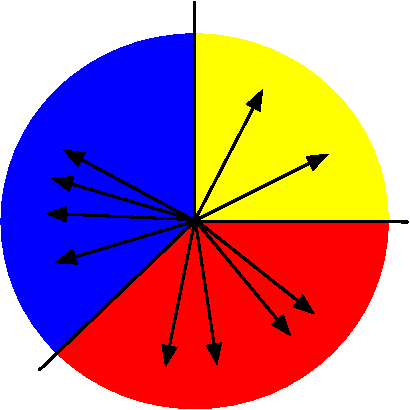
\includegraphics[scale=0.5]{ColorMap}
    \caption{The colors assigned to each displacement direction. Points with displacements along the black lines between regions will be colored so as to ensure the boundary satisfies the requirements of Sperner's Lemma.}
    \label{fig:colorMap}
  \end{figure}

  \begin{figure}
    \centering
    \begin{subfigure}[h]{0.7\textwidth}
      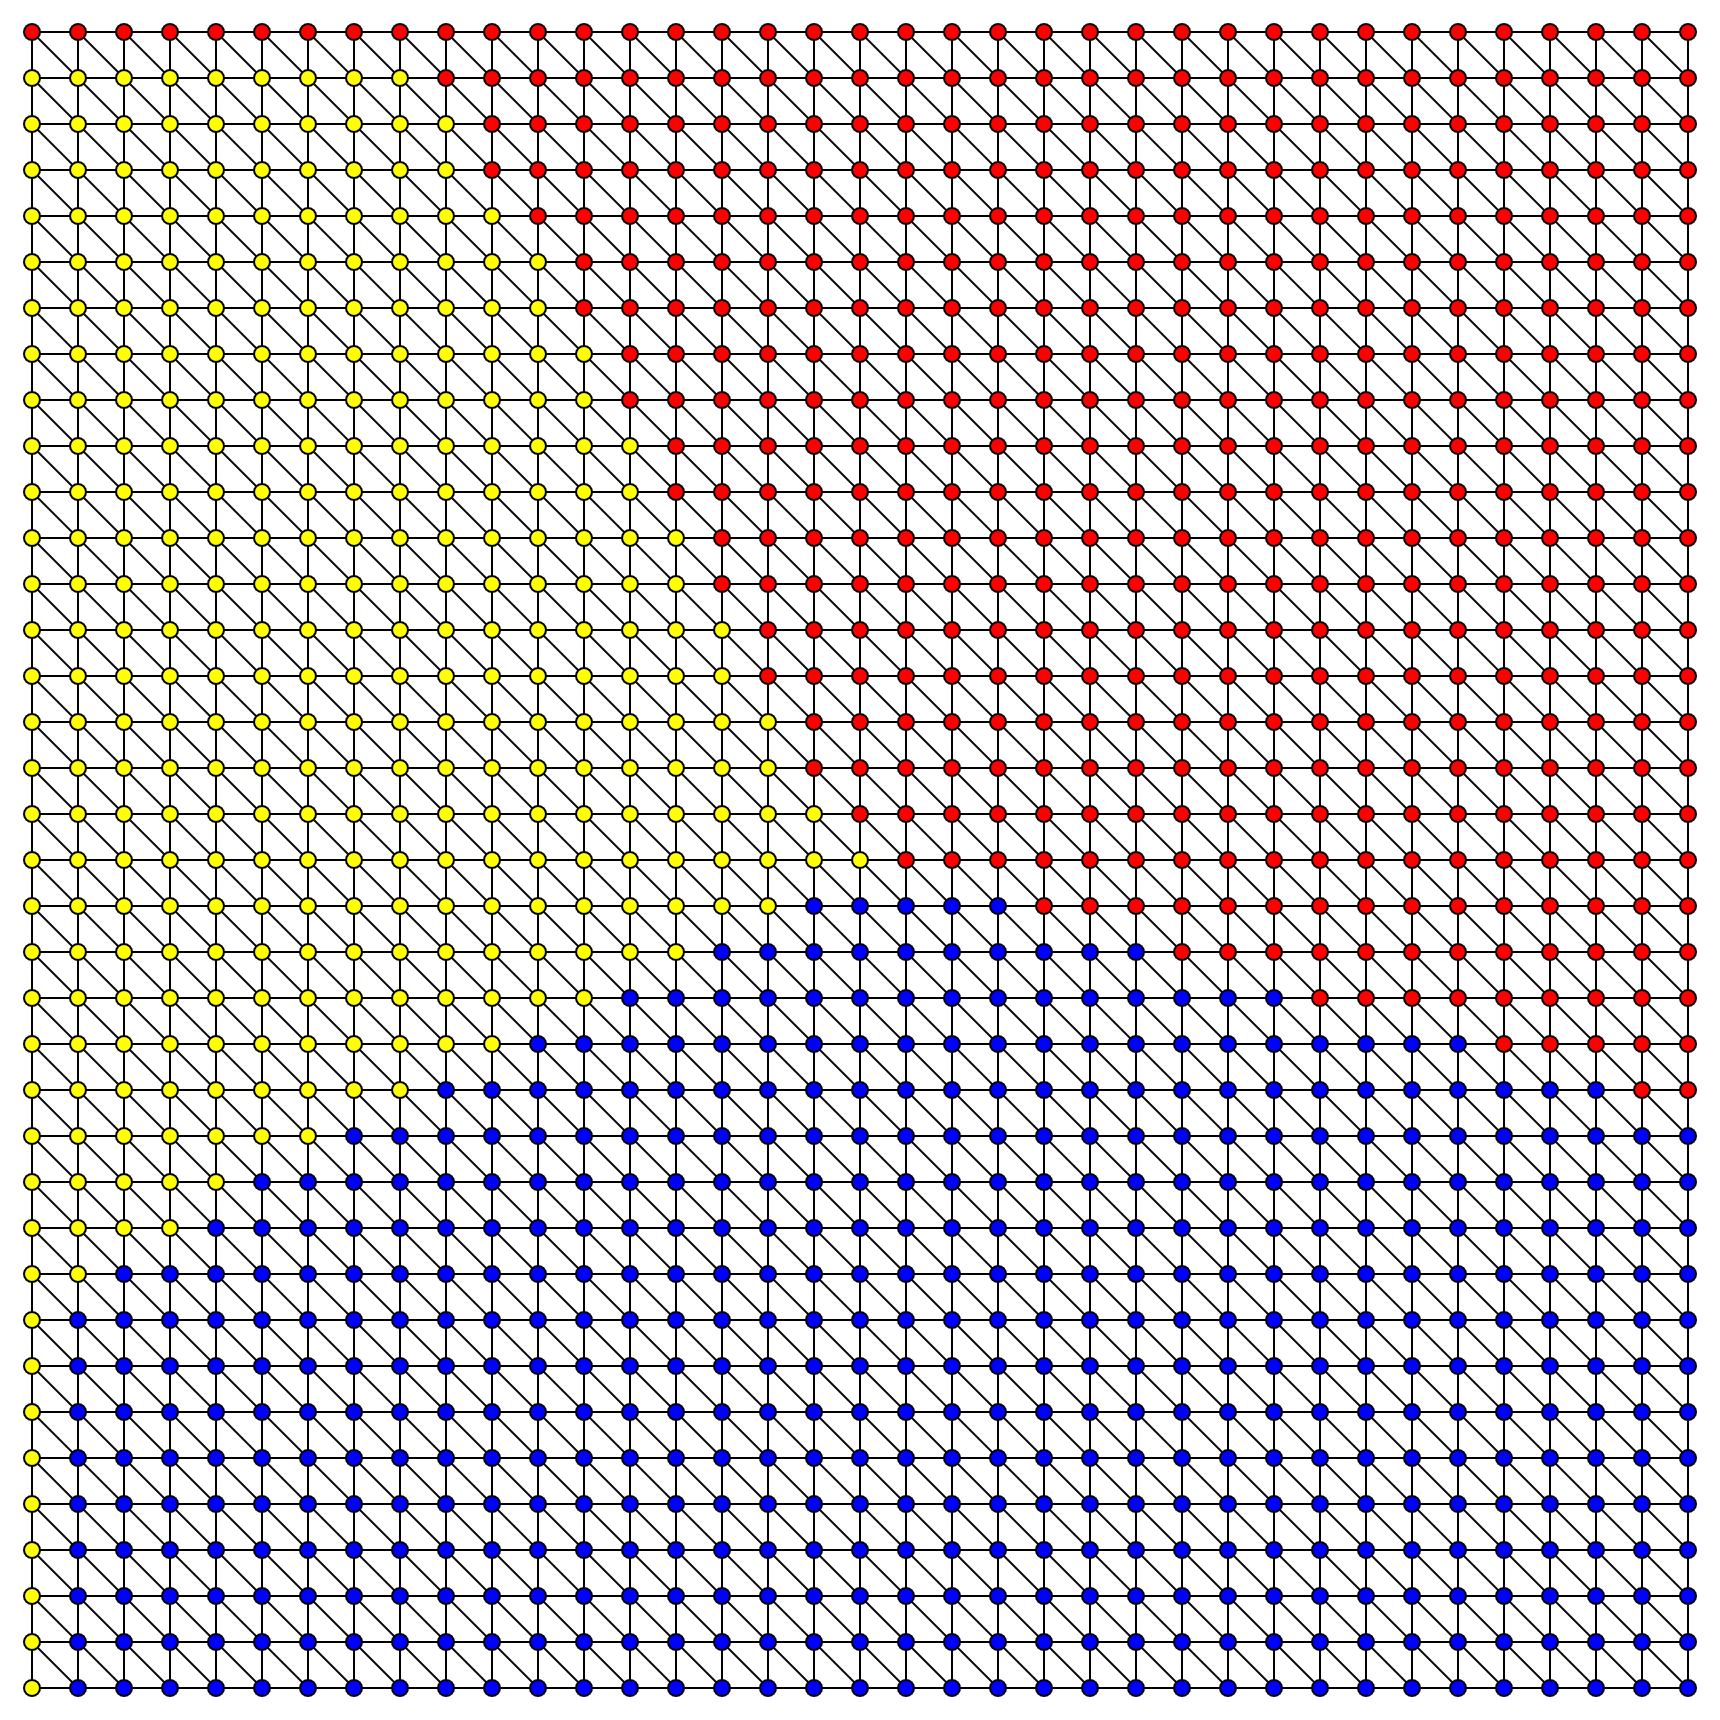
\includegraphics[width=\textwidth]{ContractionToEOPL_example1_WithoutBorder}
      \caption{A coloring for a contraction map without an added border.}
      \label{fig:withoutBorder}
    \end{subfigure}
    \begin{subfigure}[h]{0.7\textwidth}
      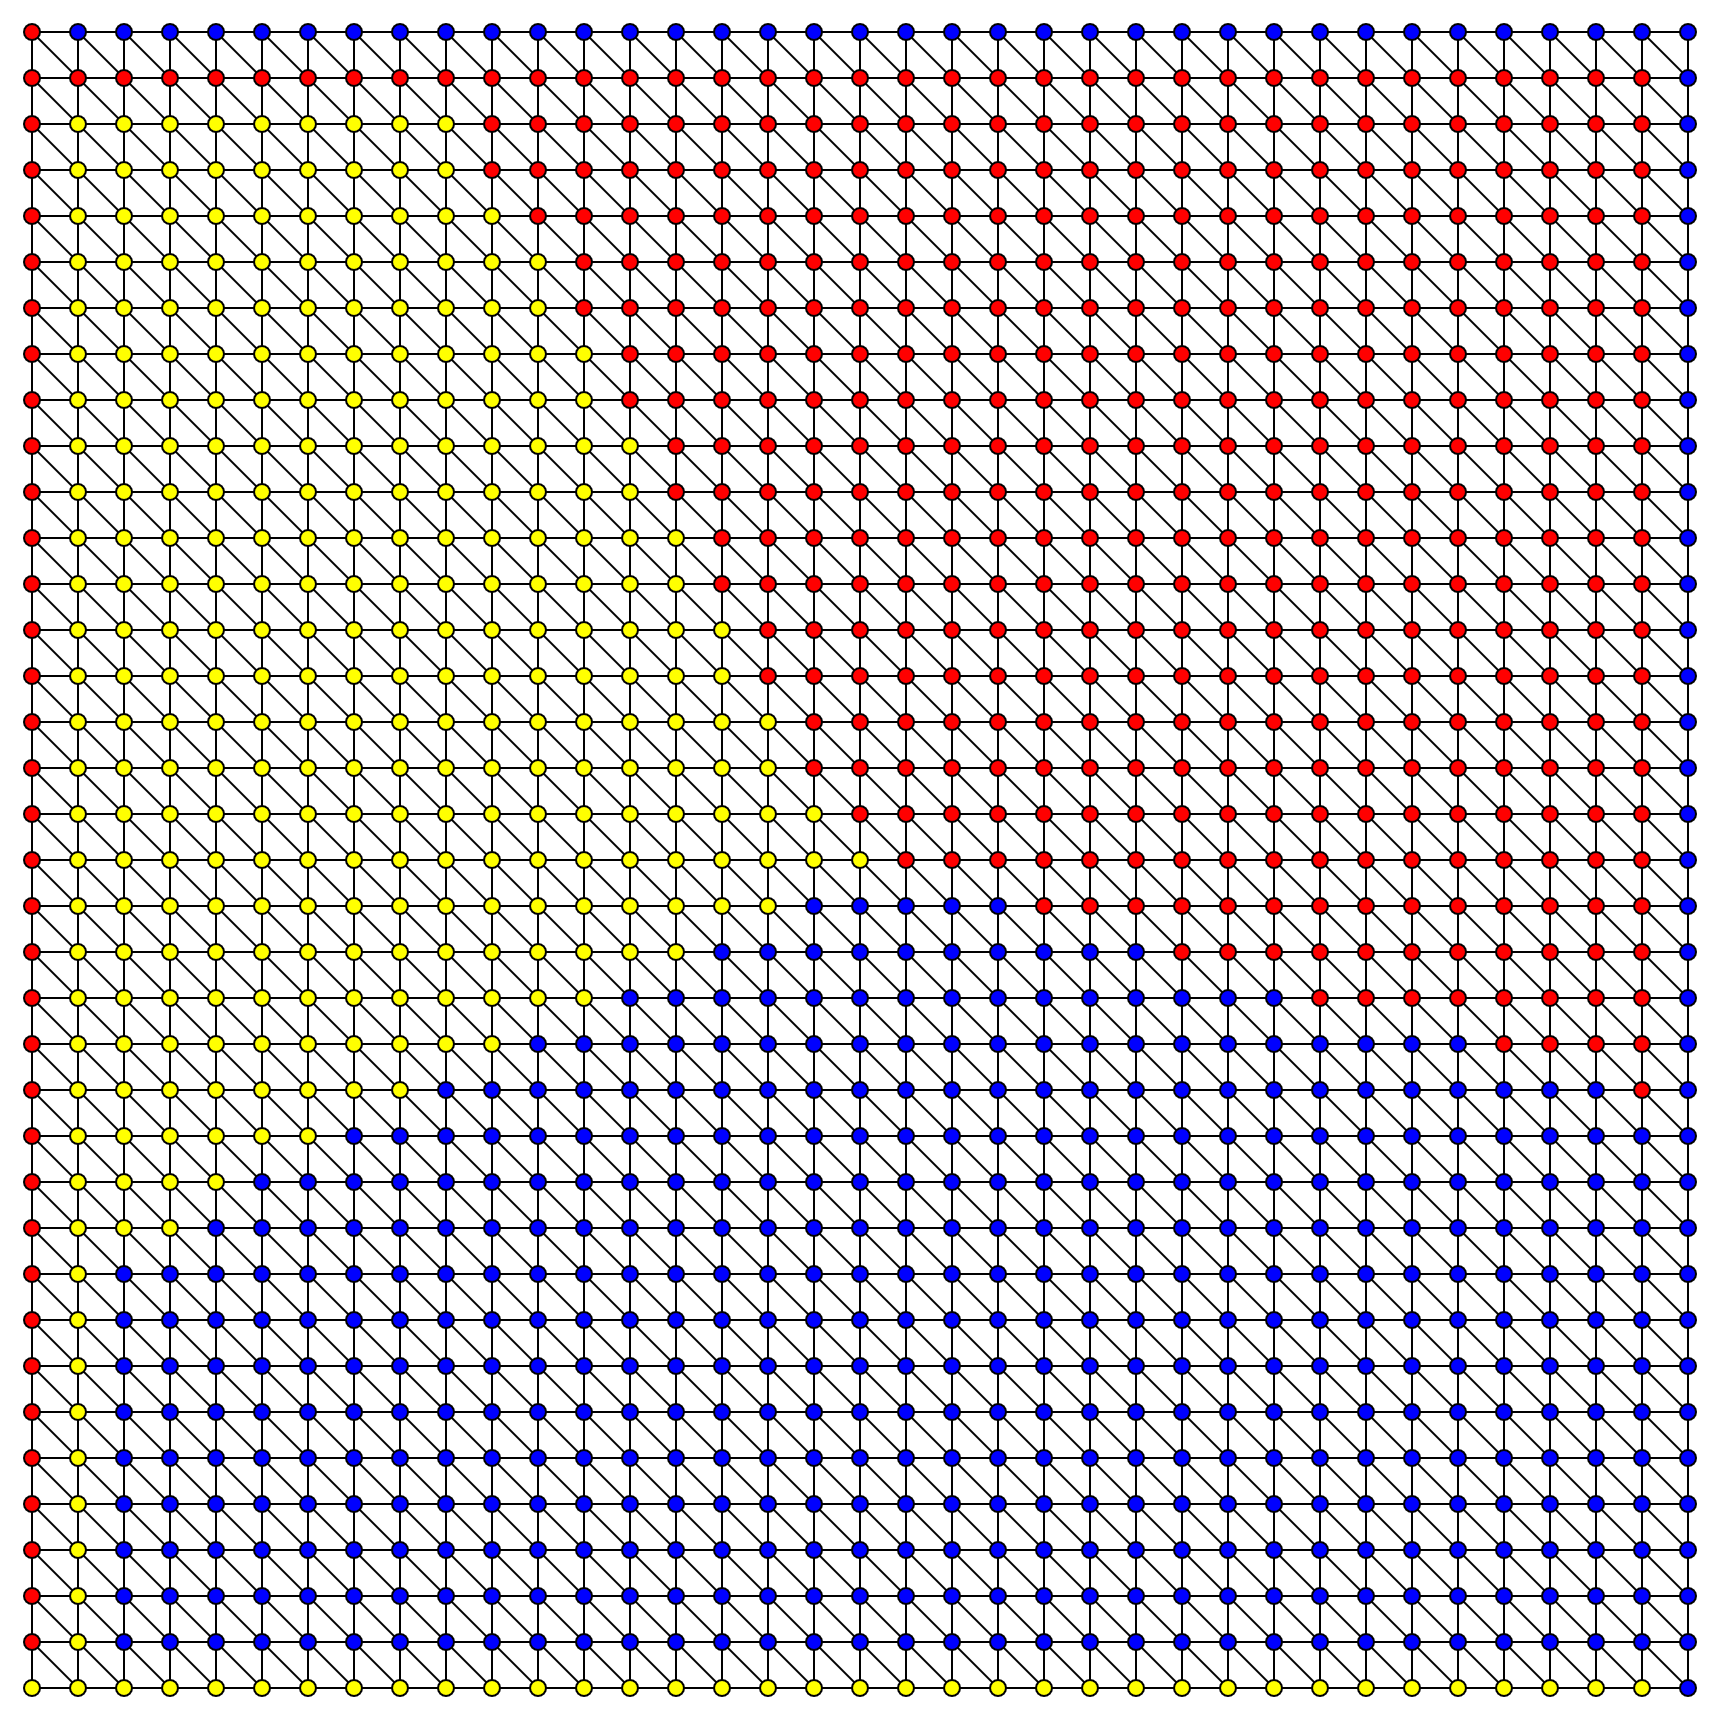
\includegraphics[width=\textwidth]{ContractionToEOPL_example1_WithBorder}
      \caption{A coloring for a contraction map with an added border.}
      \label{fig:withBorder}
    \end{subfigure}    
    \caption{Example colorings for a contraction map with and without an added border.}
    \label{fig:withAndWithoutBorder}
  \end{figure}


  \begin{figure}[h] 
    \caption{Coloring for a contraction map with displacement vectors shown at each non-boundary point.}
    \centering
    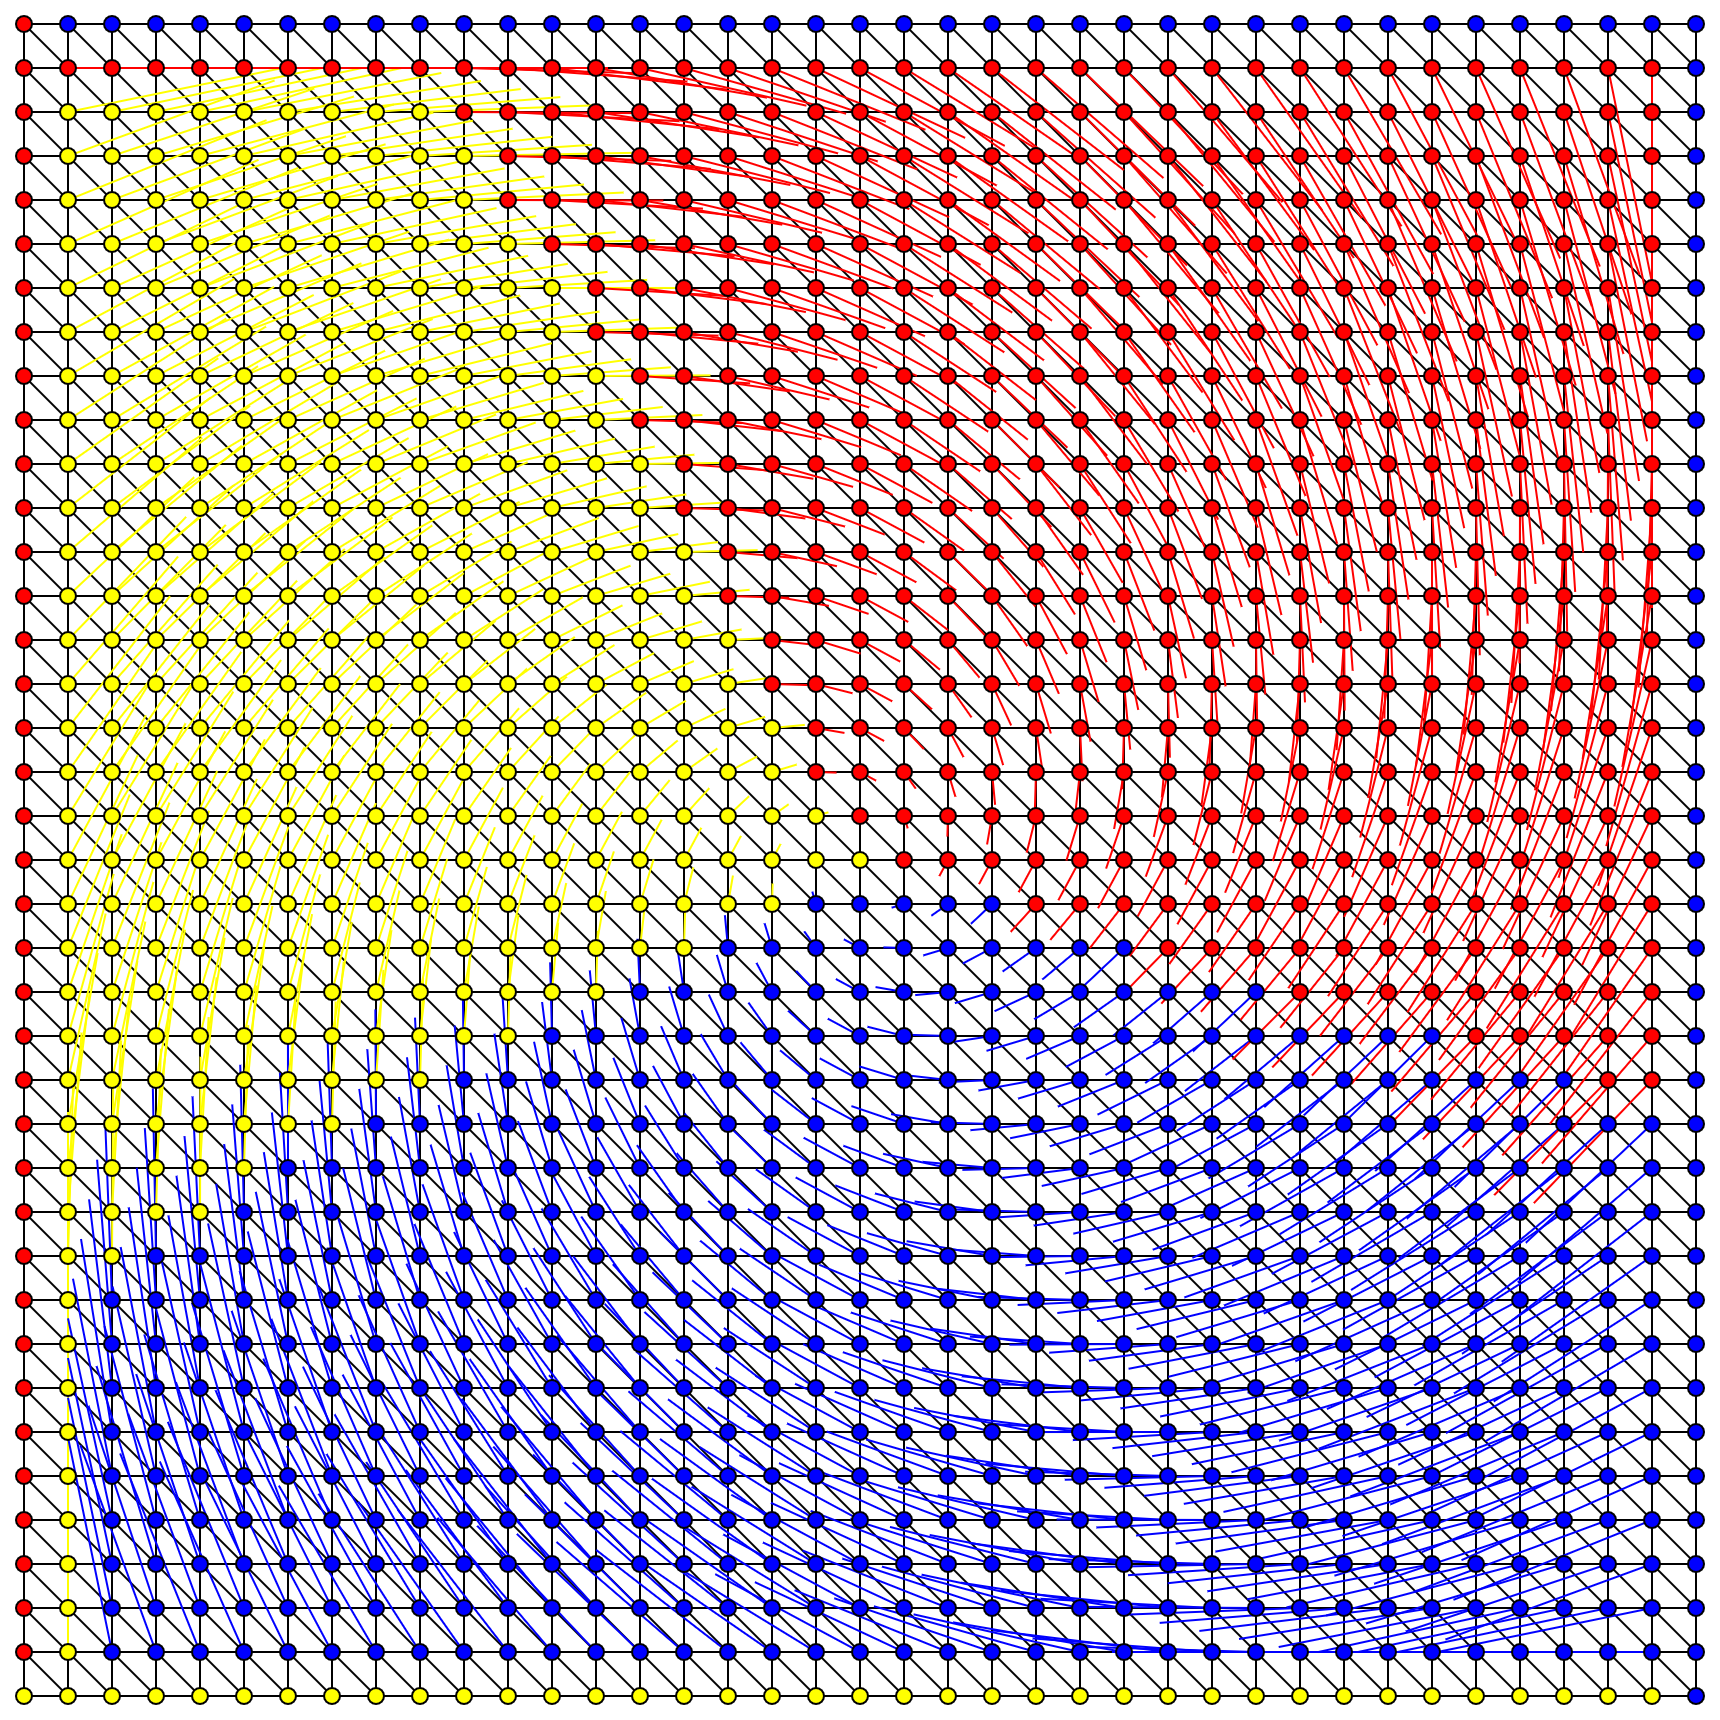
\includegraphics[width=0.7\textwidth]{ContractionToEOPL_example1_displacement}
    \label{fig:displacement}
  \end{figure}

  We assign colors from $\Set{\Yellow, \Blue, \Red}$ as follows:
  \begin{algo}
    $\mycolor(z)$:\+
    \\ \AlgoComment{Boundary Coloring}
    \\ \IfB $z_1 = -1/n$ \textbf{and} $z_2 \neq -1/n$:\+
    \\   \ReturnB $\Red$\-
    \\ \ElseIfB $z_2 = -1/n$ \textbf{and} $z_1 \neq (n+1)/n$:\+
    \\   \ReturnB $\Yellow$\-
    \\ \ElseIfB $z_2 = (n+1)/n$ \textbf{or} $z_1 = (n+1)/n$:\+
    \\   \ReturnB $\Blue$\-
    \\
    \\ \AlgoComment{Interior Coloring}
    \\ \IfB $\theta(f(z) - z) \in [0, \pi/2]$:\+
    \\   \IfB $z_1 = 1$:\+
    \\     \ReturnB $\Blue$\-
    \\   \ElseIfB $z_2 = 1$:\+
    \\     \ReturnB $\Red$\-
    \\   \ElseB:\+
    \\     \ReturnB $\Yellow$\-\-
    \\ \ElseIfB $\theta(f(z) - z) \in (\pi/2, 5\pi/4)$:\+
    \\   \ReturnB $\Blue$\-
    \\ \ElseIfB:\+
    \\   \ReturnB $\Red$\-\-
  \end{algo}

  Let $\mycolor\restr_{\DomInt} : \DomInt \to \Set{\Blue, \Red, \Yellow}$ denote the restriction of $\mycolor$ to $\DomInt$. The following lemma is immediate:
  \begin{lemma}
    $\mycolor\restr_{\DomInt}$ is a legal coloring of $\DomInt$ for any function $f: [0,1]^2\to [0,1]^2$
  \end{lemma}

  Moreover, the border coloring doesn't introduce any trichromatic triangle. As a result, we have that
  \begin{lemma}
    There exists a trichromatic triangle $x,y,z$ under $\mycolor$ where $x,y,z\in \DomInt$, and there are no trichromatic triangles containing vertices in $\Dom\setminus \DomInt$.
  \end{lemma}

  Furthermore, any trichromatic triangle entirely contained in $\DomInt$ gives a solution to the starting instance $\CI$. This can be seen in the folllowing lemma, part of which appears in a similar form in \cite{scarf1967approximation}:

  \begin{lemma}
      \label{lemma:TrichromaticTriangles}
    If $z^Y,z^R,z^B \in \Delta(\DomInt)$ are yellow, red, and blue vertices, respectively, of a trichromatic triangle (not necessarily in clockwise order), then either $z^Y$ is a solution of type \ref{2dcm:fixpoint} or two of the vertices in the triangle give a solution of type \ref{2dcm:violation}.
  \end{lemma}
  \begin{proof}
    By construction, $(f(z^Y) - z^Y)_1 (f(z^B) - z^B)_1 \leq 0$ and $(f(z^Y) - z^Y)_2 (f(z^R) - z^R)_2 \leq 0$.
    If $f$ is $c$-contracting, then we have 
    \begin{align*}
      \Abs{(f(z^Y) - z^Y)_1} &\leq \Abs{(f(z^Y) - z^Y)_1 - (f(z^B) - z^B)_1}\\
                             &= \Abs{(f(z^Y) - f(z^B))_1 + (z^B - z^Y)_1}\\
                             &\leq \Abs{(f(z^Y) - f(z^B))_1} + \Abs{(z^Y - z^B)_1}\\
                             &\leq \Norm{(f(z^Y) - f(z^B))_1} + \Norm{(z^Y - z^B)}\\
                             &\leq (c+1)\Norm{(z^Y - z^B)_1}\\
                             &\leq 4\e\\
                             &\leq \delta/2^{1/p}
    \end{align*}  and by an analogous argument, we have
    \[ \Abs{(f(z^Y) - z^Y)_2} \leq \delta/2^{1/p}\text{.} \]

    If either of these fails to hold, then the corresponding pair of points is a solution of type \ref{2dcm:violation}.

    If both hold, then we have
    \begin{align*}
      \Norm{f(z^Y) - z^Y}_p &= \Paren{\Abs{(f(z^Y) - z^Y)_1}^p + \Abs{(f(z^Y) - z^Y)_2}^p}^{1/p} \\
                          &\leq \Paren{\delta^p/2 + \delta^p/2}^{1/p}\\
                          &\leq \delta
    \end{align*} and $z^Y$ is a solution of type \ref{2dcm:fixpoint}.
  \end{proof}

  Before defining the \EOPL instance from this coloring, we make the key observation needed to get a valid potential function: If $f$ is a valid contraction map (with any constant $c < 1$), there is no yellow point above a red point, i.e., there is no pair $z^Y,z^R \in D$ with $z^R = z^Y - (0,k/n)$ with $\mycolor(z^Y) = \Yellow$ and $\mycolor(z^R) = \Red$ for any $k$. 

  \begin{lemma} \label{lemma:YellowAboveRed}
    If $z^Y, z^R \in D$ with $z^R = z^Y - (0,1)/n$ such that $\mycolor(z^Y) = \Yellow$ and $\mycolor(z^R) = \Red$, then $\Norm{f(z^Y) - (z^R)}_p \geq \Norm{z^Y - z^R}_p$, and $f$ is not a contraction map.
  \end{lemma}

  \begin{proof}
    Let $z^Y$ and $z^R$ be as in the statement. By our border coloring, it cannot be the case that $z^Y_1 = -1$, $z^Y_1 = n+1$, or $z^Y_2 = n+1$. Nor can $z^R_2 = -1$. Thus, both $z^R$ and $z^Y$ must have been colored according to $\theta^Y = \theta(f(z^Y) - z^Y)$ and $\theta^R = \theta(f(z^R) - z^R)$. By construction, we have $\theta^Y \in [0,\pi/2]$ and $\theta^R \in [5\pi/4,2\pi)$. So \[ (f(z^Y) - z^Y)_2 (f(z^R) - z^R)_2 \leq 0 \] and we have
    \begin{align*}
      \Norm{f(z^R) - f(z^Y)}_p &\geq \Abs{(f(z^R) - f(z^Y))_2} \\
                               &> \Norm{z^R - z^Y}_p
    \end{align*}

    so $z^R$ and $z^Y$ are witnesses to $f$ not being $c$-contracting (or contracting at all).
  \end{proof}

  \begin{corollary} \label{corollary:LeftEdgeIsSolution}
    If $z^Y$ and $z^R$ are vertices of a triangle in $\Delta(\DomInt)$ with $\mycolor(z^Y) = \Yellow$, $\mycolor(z^R) = \Red$, and $z^Y = z^R + (0,1/n)$, then the pair $(z^Y,z^R)$ is a solution of type \ref{2dcm:violation} for $\CE$.
  \end{corollary}

  We now will construct the \EOPL instance from this coloring. Intuitively, two triangles will be adjacent if they share an edge with one $\Red$ endpoint and one $\Yellow$ endpoint. We will orient the edges of the \EOPL graph so that there is an edge from $(z^0, z^1, z^2)$ to $(w^0, w^1, w^2)$ if facing the shared $\Red$-$\Yellow$ from a point inside $(z^0, z^1, z^2)$, the $\Red$ endpoint is to the left of the $\Yellow$ endpoint. Equivalently, the edge is oriented in this way if the $\Red$ vertex immediately preceeds the $\Yellow$ vertex in a clockwise enumeration of the vertices $z^0,z^1,z^2$ (perhaps beginning with $z^1$ or $z^2$). 

  Lemma~\ref{lemma:YellowAboveRed} now implies that the \EOPL graph will never have edges from right to left if $f$ is a contraction map, since edges from right to left have a yellow top-endpoint and a red bottom-endpoint. By Corollary~\ref{corollary:LeftEdgeIsSolution}, both triangles sharing such an edge give solutions to $\CE$, so we modify the graph to make the left triangle the start of its path, and the right triangle the end of its path.

  \begin{algo}
    $\Succ(z^0,z^1,z^2)$:\+
    \\ \IfB $\exists i,j$ with $j = i + 1 \pmod{3}$ such that $\mycolor(z^i) = \Red$ and $\mycolor(z^j) = \Yellow$:\+
    \\   \IfB $z^1 = z^0 + (1,0)/n$:\quad\AlgoComment{Top-right corner triangle\+  }  
    \\     \IfB $i = 0$:\+
    \\       \ReturnB $z^0+(0,1)/n,z^1,z^0$\quad\AlgoComment{Successor is above}\-
    \\     \ElseIfB $i = 1$:\+
    \\       \ReturnB $z^1,z^2 + (1,0)/n,z^2$\quad\AlgoComment{Successor is to the right}\-
    \\     \ElseB:\quad\AlgoComment{Successor is below and to the left}\+
    \\       \ReturnB $z^0,z^2,z^0 - (0,1)/n$\-\-
    \\   \ElseB:\quad\AlgoComment{Bottom-left corner triangle}\+
    \\     \IfB $i = 0$:\quad\AlgoComment{Successor is above and to the right}\+
    \\       \ReturnB $z^0,z^0+(1,0)/n,z^1$\-
    \\     \ElseIfB $i = 1$:\quad\AlgoComment{Successor is below}\+
    \\       \ReturnB $z^2,z^1,z^1-(0,1)/n$\-
    \\     \ElseB: \quad\AlgoComment{We have a violation of contraction by Lemma \ref{lemma:YellowAboveRed}}\+
    \\       \ReturnB $z^0,z^1,z^2$\quad\AlgoComment{Make this the end of a line}\-\-\-
    \\ \ReturnB $z^0,z^1,z^2$\quad\AlgoComment{Make a self-loop if no leaving edge}
  \end{algo}
    
  \begin{algo}
    $\Pred(z^0,z^1,z^2)$:\+
    \\ \IfB $\exists i,j$ with $j = i + 1 \pmod{3}$ such that $\mycolor(z^i) = \Yellow$ and $\mycolor(z^j) = \Red$:\+
    \\   \IfB $z^1 = z^0 + (1,0)/n$:\quad // Top-right corner triangle\+    
    \\     \IfB $i = 0$:\quad Predecessor is above\+
    \\       \ReturnB $z^0+(0,1)/n,z^1,z^0$\-
    \\     \ElseIfB $i = 1$: \quad// We have a violation of contraction by Lemma \ref{lemma:YellowAboveRed}\+
    \\       \ReturnB $z^0,z^1,z^2$ \quad// Make this the start of a line\-
    \\     \ElseB:\quad // Predecessor is below and to the left\+
    \\       \ReturnB $z^0,z^2,z^0 - (0,1)/n$\-\-
    \\   \ElseB:\quad // Bottom-left corner triangle\+
    \\     \IfB $i = 0$:\quad // Predecessor is above and to the right\+
    \\       \ReturnB $z^0,z^0+(1,0)/n,z^1$\-
    \\     \ElseIfB $i = 1$:\quad // Predecessor is below\+ 
    \\       \ReturnB $z^2,z^1,z^1-(0,1)/n$\-
    \\     \ElseB:\quad // Predecessor is to the left\+
    \\       \ReturnB $z^0-(1,0)/n,z^0,z^2$\-\-\-
    \\ \ReturnB $z^0,z^1,z^2$ \quad// Make a self-loop if no entering edge
  \end{algo}
  
  Having removed all right-to-left edges from the \EOPL graph, we'll be able to upper bound the length of the Sperner path starting in the bottom left triangle to get to any triangle in $\Delta(\Dom)$. We can then use this upper bound to assign potentials to each triangle that are guaranteed to be greater than any potential in a previous triangle along that path.

  We will set a triangle's potential to the length of the longest path that could have possibly led to this triangle. To that end, the potential of a triangle $z^0,z^1,z^2$ will be the sum of the number of triangles to the left of this one, $2(n+2)(z^0_1 + 1)$, and the number of triangles ``before'' this one with top-left corners in the same column as $z^0$. This is slightly trickier than it sounds. 
  Counting the number of triangles ``before'' the triangle in question is done by determining whether the path in this column is going up or down so that we can start counting from the bottom or top, respectively. To do this we first check whether the successor of this triangle gives us enough information to determine the direction. If not, we check the predecessor. If after doing this we still don't have enough information to determine the direction of the path in this column, then this triangle must be an isolated vertex, and we can give it a dummy potential value of $0$ (which doesn't introduce solutions since any such vertex will have a self-loop).

One additional complication arises when we observe that there are two triangles sharing the same top-left corner, and we need to account for this when counting triangles before the current triangle. 
  \begin{algo}
    $\Value(z^0,z^1,z^2)$:\+
    \\  $(s^0,s^1,s^2) \gets \Succ(z^0,z^1,z^2)$
    \\  $(p^0,p^1,p^2) \gets \Pred(z^0,z^1,z^2)$
    \\  \IfB $(z^0,z^1,z^2) \neq (s^0,s^1,s^2)$:\quad\AlgoComment{Has a possible successor}\+
    \\    \IfB $z^2 = z^0 - (0,1)/n$:\quad\AlgoComment{Bottom-left corner triangle}\+
    \\      \IfB $s^0 = z^0$:\quad\AlgoComment{Successor across the diagonal}\+
    \\        \ReturnB $2(n+2)(z^0_1 + 1) + 2z^0_2$\-
    \\      \ElseB:\quad\AlgoComment{Successor is below, since there are no successors to the left}\+
    \\        \ReturnB $2(n+2)(z^0_1 + 1) + 2(n+1-z^0_2) + 1$\-\-
    \\    \ElseB:\quad\AlgoComment{Top-right corner triangle}\+
    \\      \IfB $s^0 = z^0$:\quad\AlgoComment{Successor is across the diagonal}\+
    \\        \ReturnB $2(n+2)(z^0_1 + 1) + 2(n+1-z^0_2)$\-
    \\      \ElseIfB $s^2 = z^0$:\quad\AlgoComment{Successor is above}\+
    \\        \ReturnB $2(n+2)(z^0_1 + 1) + 2z^0_2 + 1$\-\-\-
    \\ \AlgoComment{Either has no successor or is top-right corner triangle with successor to the right}
    \\  \IfB $(z^0,z^1,z^2) \neq (p^0,p^1,p^2)$:\quad\AlgoComment{Has a possible predecessor}\+
    \\    \IfB $z^2 = z^0 - (0,1)/n$:\quad\AlgoComment{Bottom-left corner triangle, must not have had successor}\+
    \\      \IfB $p^0 = z^0$:\quad\AlgoComment{Predecessor is across the diagonal}\+
    \\        \ReturnB $2(n+2)(z^0_1 + 1) + 2(n+1-z^0_2) + 1$\-
    \\      \ElseB:\quad\AlgoComment{Predecessor to the left with no successor or predecessor below}\+
    \\        \ReturnB $2(n+2)(z^0_1 + 1) + 2z^0_2$\-\-
    \\    \ElseB:\quad\AlgoComment{Top-right corner triangle with no successor or right successor}\+
    \\      \IfB $p^2 = z^0$:\quad\AlgoComment{Predecessor is above}\+
    \\        \ReturnB $2(n+2)(z^0_1 + 1) + 2(n+1-z^0_2)$\-
    \\      \ElseB:\quad\AlgoComment{Predecessor across the diagonal}\+
    \\        \ReturnB $2(n+2)(z^0_1 + 1) + 2z^0_2 + 1$\-\-\-
    \\  \ReturnB $0$\quad\AlgoComment{Isolated triangle, in a self-loop}. 
  \end{algo}

  In Figure \ref{fig:potentials}, an example coloring and associated potentials are shown.
  \begin{figure}[h]
    \caption{A coloring for a contraction map and associated potentials values.}
    \centering
    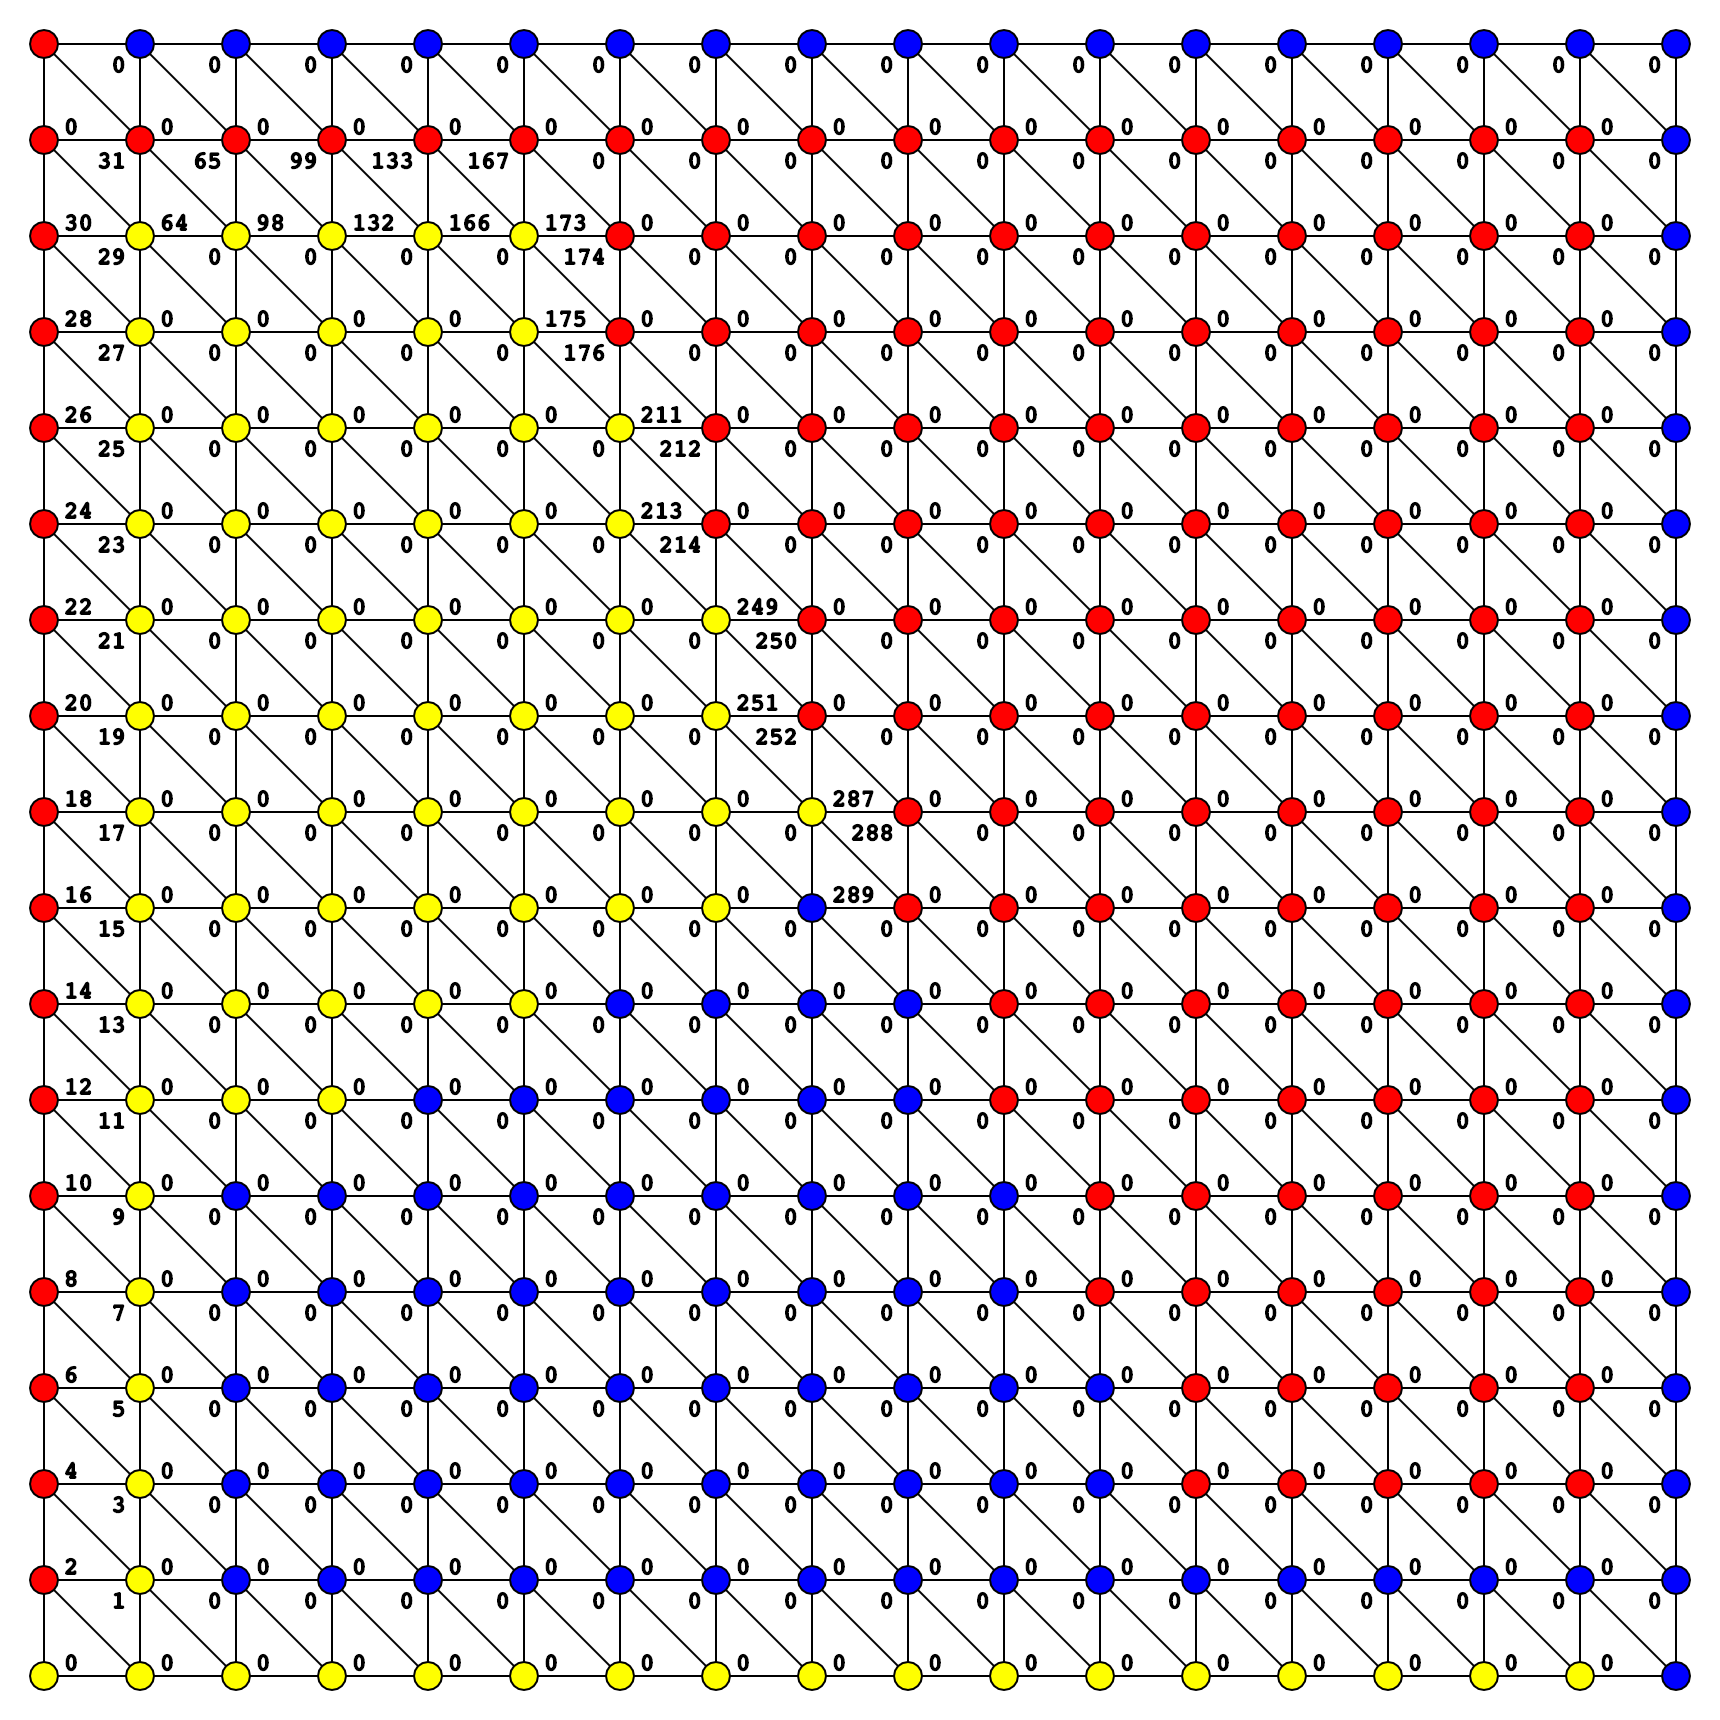
\includegraphics[width=0.9\textwidth]{ContractionToEOPL_example1_potentials}
    \label{fig:potentials}
  \end{figure}

  \begin{lemma} \label{lemma:PotentialsIncreaseAlongPaths}
    For any triangles $T_1,T_2 \in \Delta(\Dom)$ with $T_1 \neq T_2$, if $\Succ(T_1) = T_2$ and $\Pred(T_2) = T_1$, then $\Value(T_1) < \Value(T_2)$. 
  \end{lemma}

  \begin{proof}
    Since $T_1$ and $T_2$ are adjacent in the \EOPL graph, they must share a side. Furthermore, $T_2$ cannot be to the left of $T_1$ since we break all paths rather than introduce an edge to the left. Thus, there are three cases to consider:
    \begin{description}
    \item[$T_2$ is above $T_1$] In this case, the potential at $T_2$ and $T_1$ will be computed counting from the bottom of the column, and $\Value(T_2) > \Value(T_1)$.
    \item[$T_2$ is below $T_1$] In this case, the potential at $T_2$ and $T_1$ will be computed counting from the top of the column and $\Value(T_2) > \Value(T_1)$. 
    \item[$T_2$ is to the right of $T_1$] The potential of any triangle (with non-zero potential) in a given column will be greater than the potential of any triangle in any column to the left of the given column. Thus, $\Value(T_2) > \Value(T_1)$.
    \end{description}
  \end{proof}

  As a corollary of the above lemma, we get

  \begin{corollary} \label{coro:BadPotentialGiveViolations}
    There are no solutions of type \ref{eopl2:bad_potential} in the instance $\CE$ generated by our reduction.
  \end{corollary}

  \begin{lemma} \label{lemma:EndOfLineSolutions}
    Any solution $T \in \Delta(\Dom)$ of type \ref{eopl2:eol} gives a solution for the \TwoDContractionMap instance.
  \end{lemma}
  \begin{proof}
     Consider a solution $T \in \Delta(\DomInt)$ of type \ref{eopl2:eol}. By construction, every triangle without a red-yellow side is in a self-loop, so $T$ must have at least one red vertex and at least one yellow vertex. There are two cases to consider: Either $T$ also has a blue vertex, in which it is a trichromatic triangle, and gives a solution of type \ref{2dcm:fixpoint} by Lemma \ref{lemma:TrichromaticTriangles}, or two of $T$'s vertices are either red or yellow. In the latter case, one of the red-yellow sides must not correspond to a valid edge in the graph, since $T$ is the either the start or end of a line. The only red-yellow sides that don't correspond to valid edges in the graph are those that are predecessor edges to the right, or successor edges to the left. In either of those case, there is a yellow vertex above a red vertex in $T$, and by Lemma \ref{lemma:YellowAboveRed}, the yellow and red vertices witness $f$ not being a contraction map, and give a solution of type \ref{2dcm:violation}.
    \end{proof}
    
    To complete the reduction, we choose for our starting triangle the following: \[(-1/n,0),(0,-1/n),(-1/n,-1/n).\] We can immediately observe that this satisfies the requirement that it has no valid predecessor.

    Finally, we observe that all of the algorithms presented can be implemented in polynomial time in the size of the input to $\CI$, and we conclude that
    \begin{theorem}
An instance of \TwoDContractionMap can be reduced to an instance of \EOPL in polynomial time such that a solution of the former can be constructed in polynomial time from the solution of the latter. 
    \end{theorem}

    
  
  % \begin{enumerate}
  % \item As far as I can tell, there can be edges pointing up in the graph other than those induced by the boundary. I should come up with an example containing edges of that sort. 
  % \item I believe this can be generalized to \ThreeDContractionMap, since I think it will be the case that paths will be limited in a similar way, so that we can assign consistent potential values to each point. 
  % \item We can look at the DTZ paper and see if their hardness proof gives us a metric from which we could do this same reduction. Or we could modify their metric somehow and still carry out the same sort of proof.
  % Can we use the $\lambda$-Lipschitz continuity of $d$ in the DTZ definition of MetricBanach to generalize this argument to that definition. 

  % If it's the case that we're given a metric which is of the form $d(x,y) = g(\Abs{x_1-x_2},\Abs{y_1-y_2})$, where $g$ is a non-decreasing function in both arguments, then I think everything works out. We may be able to extract solutions from violations of this. (Probably not, seems too rigid a constraint.)

  % Fix the JavaScript to make sure all the colors are being computed correctly, and then update the images accordingly.

  % \end{enumerate}

  % One other interesting observation: When $f$ is in fact a contraction map, there can be at most one edge from left-to-right in any given column by Lemma \ref{lemma:YellowAboveRed}. 

  % Can we go from EOPL to a standard norm-based contraction in $n$-dimensions?

  % What is the role of uniqueness of solutions.
  

%%%%%%%%%%%%%%%%%%%%%%%%%%%%%%%%%%%%%%%%%%%%%%%%%%%%%%%%%%%%%%%%%%%%%%%%%%%%%%%
% APPENDIX
%
\appendix
\section{\EOML to \EOPL}
\label{sec:EOMLtoEOPL}

Given an instance $\CI$ of $\EOML$ defined by circuits $S,P$ and $V$ on vertex
set $\{0,1\}^n$ we are going to create an instance $\CI'$ of \EOPL with circuits
$S',P'$, and $V'$ on vertex set $\{0,1\}^{(n+1)}$, i.e., we introduce one extra bit.  
This extra bit is essentially to take care of the difference in the value of potential 
at the starting point in \EOML and \EOPL, namely $1$ and $0$ respectively. 
%starting condition of $V(0^n)=1$ while in \EOPL $0^n$ has potential zero. 

Let $k=n+1$, then we create a potential function $V':\{0,1\}^k \rightarrow
\{0,\dots,2^k-1\}$. 
The idea is to make $0^k$ the starting point with potential zero as required,
and to make all other vertices with first bit $0$ be dummy vertices with self
loops. The real graph
will be embedded in vertices with first bit $1$, i.e., of type $(1,\uu)$. Here
by $(b,\uu)\in \{0,1\}^k$, where $b\in \{0,1\}$ and $\uu\in \{0,1\}^n$, we mean
a $k$ length bit string with first bit set to $b$ and for each $i\in[2:k]$ bit $i$ 
set to bit $u_i$. %Given $(b,\uu)\in \{0,1\}^k$, do the following:

\medskip
\medskip

\noindent{\bf Procedure $V'(b,\uu)$:} If $b=0$ then Return $0$, otherwise Return $V(\uu)$. 
\medskip
\medskip

\noindent{\bf Procedure $S'(b,\uu)$:}
\vspace{-0.3cm}

\begin{enumerate}
\item If $(b,\uu)=0^k$ then Return $(1,0^n)$
\item If $b=0$ and $\uu\neq 0^n$ then Return $(b,\uu)$ (creating self loop for dummy vertices)
\item If $b=1$ and $V(\uu)=0$ then Return $(b,\uu)$ (vertices with zero potentials have self loops)
\item If $b=1$ and $V(\uu)>0$ then Return $(b,S(\uu))$ (the rest follows $S$)
\end{enumerate}

\noindent{\bf Procedure $P'(b,\uu)$:}
\vspace{-0.3cm}

\begin{enumerate}
\item If $(b,\uu)=0^k$ then Return $(b,\uu)$ (initial vertex points to itself in $P'$).
\item If $b=0$ and $\uu\neq 0^n$ then Return $(b,\uu)$ (creating self loop for dummy vertices)
\item If $b=1$ and $\uu=0^n$ then Return $0^k$ (to make $(0,0^n)\rightarrow (1,0^n)$ edge consistent)
\item If $b=1$ and $V(\uu)=0$ then Return $(b,\uu)$ (vertices with zero potentials have self loops)
\item If $b=1$ and $V(\uu)>0$ and $\uu \neq 0^n$ then Return $(b,P(\uu))$ (the rest follows $P$)
\end{enumerate}

Valid solutions of \EOML of type T2 and T3 requires the potential to be strictly greater than zero, while solutions of \EOPL may have zero potential. However, a solution of \EOPL can not be a self loop, so we've added self-loops around vertices with zero potential in the \EOPL instance.
By construction, the next lemma follows:
\begin{lemma}\label{lem:m2p-valid}
$S'$, $P'$, $V'$ are well defined and polynomial in the sizes of $S$, $P$, $V$ respectively. 
\end{lemma}

Our main theorem in this section is a consequence of the following three lemmas.

\begin{lemma}\label{lem:m2p-sl}
For any $\xx=(b,\uu)\in \{0,1\}^k$, $P'(\xx)=S'(\xx)=\xx$ (self loop) iff $\xx\neq 0^k$, and $b=0$ or $V(\uu)=0$.
\end{lemma}
\begin{proof}
This follows by the construction of $V'$, the second condition in $S'$ and $P'$, and third and fourth conditions in $S'$ and $P'$ respectively. 
\end{proof}

\begin{lemma}\label{lem:m2p-r1}
Let $\xx=(b,\uu)\in \{0,1\}^k$ be such that $S'(P'(\xx))\neq \xx \neq 0^k$ or $P'(S'(\xx))\neq \xx$ (an R1 type solution of \EOPL instance $\CI'$), then $\uu$ is a solution of \EOML instance $\CI$.
\end{lemma}
\begin{proof}
The proof requires a careful case analysis. 
By the first conditions in the descriptions of $S',P'$ and $V'$, we have $\xx \neq 0^k$. 
Further, since $\xx$ is not a self loop, Lemma \ref{lem:m2p-sl} implies $b=1$  and $V'(1,\uu)=V(\uu)>0$.
\medskip

\noindent{\em Case I.}
If $S'(P'(\xx))\neq \xx\neq 0^k$ then we will show that either $\uu$ is a genuine start of a line other than $0^n$ giving a T1 type solution of \EOML instance $\CI$, or there is some issue with the potential at $\uu$ giving either a T2 or T3 type solution of $\CI$. Since $S'(P'(1,0^n))=(1,0^n)$, $\uu \neq 0^n$. Thus if $S(P(\uu))\neq \uu$ then we get a T1 type solution of $\CI$ and proof follows. If $V(\uu)=1$ then we get a T2 solution of $\CI$ and proof follows. 

Otherwise, we have $S(P(\uu))=\uu$ and $V(\uu)>1$. Now since also $b=1$ $(1,\uu)$ is not a self loop (Lemma \ref{lem:m2p-sl}). %and $S'(P'(b,\uu))\neq (b,\uu)$, we have that $(1,\uu)$ is not a selfloop. 
Then it must be the case that $P'(1,\uu)=(1,P(\uu))$. However, $S'(1,P(\uu))\neq (1,\uu)$ even though $S(P(\uu))=\uu$. This happens only when $P(\uu)$ is a self loop because of $V(P(\uu))=0$ (third condition of $P'$).
Therefore, we have $V(\uu)-V(P(\uu))>1$ implying that $\uu$ is a T3 type solution of $\CI$. 
\medskip

\noindent{\em Case II.}
Similarly, if $P'(S'(\xx))\neq \xx$, then either $\uu$ is a genuine end of a line of $\CI$, or there is some issue with the potential at $\uu$. If $P(S(\uu))\neq \uu$ then we get T1 solution of $\CI$. Otherwise, $P(S(\uu))=\uu$ and $V(\uu)>0$. Now as $(b,\uu)$ is not a self loop and $V(\uu)>0$, it must be the case that $S'(b,\uu)=(1,S(\uu))$. However, $P'(1, S(\uu))\neq (b,\uu)$ even though $P(S(\uu))=\uu$. This happens only when $S(\uu)$ is a self loop because of $V(S(\uu))=0$. Therefore, we get $V(S(\uu))-V(\uu)<0$, i.e., $\uu$ is a type T3 solution of $\CI$. 
\end{proof}

\begin{lemma}\label{lem:m2p-r2}
Let $\xx=(b,\uu)\in \{0,1\}^k$ be an R2 type solution of the constructed \EOPL instance $\CI'$, then $\uu$ is a type T3 solution of \EOML instance~$\CI$.
\end{lemma}
\begin{proof}
Clearly, $\xx\neq 0^k$. Let $\yy = (b',\uu') = S'(\xx) \neq \xx$, and observe that $P(\yy) = \xx$. This also implies that $\yy$ is not a self loop, and hence $b=b'=1$ and $V(\uu)>0$ (Lemma \ref{lem:m2p-sl}). Further, $\yy = S'(1,\uu)=(1,S(\uu))$, hence $\uu'=S(\uu)$. Also, $V'(\xx)=V'(1,\uu)=V(\uu)$ and $V'(\yy)=V'(1,\uu')=V(\uu')$. 

Since $V'(\yy)-V'(\xx)\le 0$ we get $V(\uu')-V(\uu)\le 0 \Rightarrow V(S(\uu)) - V(\uu) \le 0\Rightarrow V(S(\uu)) - V(\uu)\neq 1$. Given that $V(\uu)>0$, $\uu$ gives a type T3 solution of \EOML.
\end{proof}

\begin{theorem}\label{thm:m2p}
An instance of \EOML can be reduced to an instance of \EOPL in linear time such that a solution of the former can be constructed in a linear time from the solution of the latter. 
\end{theorem}


\section{\EOPL to \EOML}
\label{sec:eopl2eoml}

In this section we give a linear time reduction from an instance $\CI$ of \EOPL to an instance $\CI'$ of \EOML. Let the given \EOPL instance $\CI$ be defined on vertex set $\{0,1\}^n$ and with procedures $S,P$ and $V$, where $V:\{0,1\}^n\rightarrow \{0,\dots,2^m-1\}$. 
\medskip

\noindent{\bf Valid Edge.} We call an edge $\uu \rightarrow \vv$ valid if $\vv=S(\uu)$ and $\uu=P(\vv)$. 
\medskip

We construct an \EOML instance $\CI'$ on $\{0,1\}^k$ vertices where $k=n+m$. 
Let $S',P'$ and $V'$ denotes the procedures for $\CI'$ instance. 
The idea is to capture value $V(\xx)$ of the potential in the $m$ least significant bits of vertex description itself, so that it can be gradually increased or decreased on valid edges. For vertices with irrelevant values of these least $m$ significant bits we will create self loops. Invalid edges will also become self loops, e.g., if $\yy=S(\xx)$ but $P(\yy)\neq \xx$ then set $S'(\xx,.)=(\xx,.)$. We will see how these can not introduce new solutions. 

%
In order to ensure $V'(0^k)=1$, the $V(S(0^n))=1$ case needs to be discarded. For
this, we first do some initial checks to see if the given instance $\CI$ is not
trivial.  If the input \EOPL instance is trivial, in the sense that either
$0^n$ or $S(0^n)$ is a solution, then we can just return it.

\begin{lemma}
\label{lem:valid-edges}
If $0^n$ or $S(0^n)$ are not solutions of \EOPL instance $\CI$ then $0^n
\rightarrow S(0^n) \rightarrow S(S(0^n))$ are valid edges, and $V(S(S(0^n))\ge 2$. 
\end{lemma}

\begin{proof}
Since both $0^n$ and $S(0^n)$ are not solutions, we have
	$V(0^n)<V(S(0^n))<V(S(S(0^n)))$, $P(S(0^n))=0^n$, and for $\uu = S(0^n)$,
	$S(P(\uu))=\uu$ and $P(S(\uu))=\uu$. In other words, $0^n \rightarrow S(0^n)
	\rightarrow S(S(0^n))$ are valid edges, and since $V(0^n)=0$, we have
	$V(S(S(0^n))\ge 2$. 
\end{proof}

%In $\CI'$ we want $V'(0^k)=1$. Therefore if $V(S(0^n))=1$ then it will interfer. 
Let us assume now on that $0^n$ and $S(0^n)$ are not solutions of $\CI$, and
then by Lemma \ref{lem:valid-edges}, we have $0^n \rightarrow S(0^n) \rightarrow
S(S(0^n))$ are valid edges, and $V(S(S(0^n))\ge 2$. We can avoid the need to check
whether $V(S(0))$ is one all together, by making $0^n$ point directly to
$S(S(0^n))$ and make $S(0^n)$ a dummy vertex. 

We first construct $S'$ and $P'$, and then construct $V'$ which will give
value zero to all self loops, and use the least significant $m$ bits to give a
value to all other vertices.
%\medskip
Before describing $S'$ and $P'$ formally, we first describe the underlying
principles. Recall that in $\CI$ vertex set is $\{0,1\}^n$ and possible potential values are $\{0,\dots,2^m-1\}$, while in $\CI'$ vertex set is $\{0,1\}^k$ where $k=m+n$. 
We will denote a vertex of $\CI'$ by a tuple $(\uu,\pi)$, where $\uu \in
\{0,1\}^n$ and $\pi\in \{0,\dots,2^m-1\}$. 
Here when we say that we introduce an {\em edge $\xx\rightarrow \yy$} we mean
that we introduce a valid edge from $\xx$ to $\yy$, i.e., $\yy=S'(\xx)$ and $\xx=P(\yy)$. 
%In what follows, let $(\uu,\pi)$ be a given vertex of $\CI'$. 
\begin{itemize}
\item Vertices of the form $(S(0^n),\pi)$ for any $\pi \in \{0,1\}^m$ and the vertex $(0^n,1)$ are
dummies and hence have self loops.
\item If $V(S(S(0^n))=2$ then we introduce an edge $(0^n,0)\rightarrow(S(S(0^n)),2)$, otherwise 
\begin{itemize}
\item for $p=V(S(S(0^n))$, we introduce the edges $(0^n,0)\ra (0^n,2)\ra (0^n, 3)\dots (0^n,p-1)\ra (S(S(0^n)),p)$.
\end{itemize}
\item If $\uu \ra \uu'$ valid edge in $\CI$ then let $p=V(\uu)$ and $p'=V(\uu')$
\begin{itemize}
\item If $p=p'$ then we introduce the edge $(\uu,p)\ra (\uu',p')$. %, and the rest of $(\uu,\pi),\ \forall \pi\neq p'$ are self loop.
\item If $p<p'$ then we introduce the edges $(\uu,p)\ra (\uu,p+1)\ra \dots\ra (\uu,p'-1)\ra (\uu',p')$.
\item If $p>p'$ then we introduce the edges $(\uu,p)\ra (\uu,p-1)\ra \dots\ra (\uu,p'+1)\ra (\uu',p')$.
\end{itemize}
\item If $\uu\neq 0^n$ is the start of a path, i.e., $S(P(\uu))\neq \uu$, then
make $(\uu,V(\uu))$ start of a path by ensuring $P'(\uu,V(\uu))=(\uu,V(\uu))$.
\item If $\uu$ is the end of a path, i.e., $P(S(\uu))\neq \uu$, then make
$(\uu,V(\uu))$ end of a path by ensuring $S'(\uu,V(\uu))=(\uu,V(\uu))$.
\end{itemize}

Last two bullets above remove singleton solutions from the system by making them
self loops. However, this can not kill all the solutions since there is a path
starting at $0^n$, which has to end somewhere. Further, note that this entire process ensures that no new start or end of a paths are introduced. 
%does not introduce extra solutions, which would be the start or end of a
%different path. 
\medskip
\medskip

\noindent{\bf Procedure $S'(\uu,\pi)$.} %Let $\xx=(\uu,\pi)$ for notational convenience.
\vspace{-0.2cm}

\begin{enumerate}
\item If ($\uu=0^n$ and $\pi=1$) or $\uu=S(0^n)$ then Return $(\uu,\pi)$. 
\item If $(\uu,\pi)=0^k$, then let $\uu'=S(S(0^n))$ and $p'=V(\uu')$. 
\begin{enumerate}
\item If $p'=2$ then Return $(\uu',2)$ else Return $(0^n,2)$.
\end{enumerate}
\item If $\uu=0^n$ then
\begin{enumerate}
\item If $2\le \pi<p'-1$ then Return $(0^n,\pi+1)$.
\item If $\pi=p'-1$ then Return $(S(S(0^n)),p')$.
\item If $\pi\ge p'$ then Return $(\uu,\pi)$.
\end{enumerate}
%\item If $\uu=0^n$ and $\pi=1$ then Return $(0^n,1)$. 
%\item If $\uu=S(0^n)$ then Return $(\uu,\pi)$.
\item Let $\uu'=S(\uu)$, $p'=V(\uu')$, and $p=V(\uu)$. 
%\item If $\uu'=\uu$ then Return $(\uu,\pi)$.
%\item If $P(\uu')\neq \uu$ then Return $(\uu,\pi)$. 
\item If $P(\uu')\neq \uu$ or $\uu'=\uu$ then Return $(\uu,\pi)$
\item If $\pi=p=p'$ or ($\pi=p$ and $p'=p+1$) or $(\pi=p$ and $p'=p-1$) then Return $(\uu',p')$.
\item If $\pi<p\le p'$ or $p\le p'\le \pi$ or $\pi>p\ge p'$ or $p\ge p'\ge \pi$ then Return $(\uu,\pi)$
\item If $p<p'$, then If $p\le \pi<p'-1$ then Return $(\uu,\pi+1)$. If $\pi=p'-1$ then Return $(\uu',p')$.
\item If $p>p'$, then if $p \ge \pi>p'+1$ then Return $(\uu,\pi-1)$. If $\pi=p'+1$ then Return $(\uu',p')$.
\end{enumerate}
\medskip

\noindent{\bf Procedure $P'(\uu,\pi)$.} %Let $\xx=(\uu,\pi)$ for notational convenience.
\vspace{-0.2cm}

\begin{enumerate}
\item If ($\uu=0^n$ and $\pi=1$) or $\uu=S(0^n)$ then Return $(\uu,\pi)$. 
\item If $\uu=0^n$, then 
\begin{enumerate}
\item If $\pi=0$ then Return $0^k$.
\item If $\pi<V(S(S(0^n)))$ and $\pi\notin \{1,2\}$ then Return $(0^n,\pi-1)$.
\item If $\pi<V(S(S(0^n)))$ and $\pi=2$ then Return $0^k$.
\end{enumerate}
\item If $\uu=S(S(0^n))$ and $\pi=V(S(S(0^n))$ then 
\begin{enumerate}
\item If $\pi=2$ then Return $(0^n,0)$, else Return $(0^n,\pi-1)$. 
\end{enumerate}
\item If $\pi=V(\uu)$ then 
\begin{enumerate}
\item Let $\uu'=P(\uu)$, $p'=V(\uu')$, and $p=V(\uu)$. 
\item If $S(\uu')\neq \uu$ or $\uu'=\uu$ then Return $(\uu,\pi)$
\item If $p=p'$ then Return $(\uu',p')$ 
\item If $p'<p$ then Return $(\uu',p-1)$ else Return $(\uu',p+1)$
\end{enumerate}
\item Else \% when $\pi \neq V(\uu)$
\begin{enumerate}
\item Let $\uu'=S(\uu)$, $p'=V(\uu')$, and $p=V(\uu)$
\item If $P(\uu')\neq \uu$ or $\uu'=\uu$ then Return $(\uu,\pi)$
\item If $p'=p$ or $\pi<p< p'$ or $p<p'\le \pi$ or $\pi>p> p'$ or $p>p'\ge \pi$ then Return $(\uu,\pi)$
\item If $p<p'$, then If $p<\pi\le p'-1$ then Return $(\uu,\pi-1)$. 
\item If $p>p'$, then if $p> \pi\ge p'+1$ then Return $(\uu,\pi+1)$. 
\end{enumerate}
\end{enumerate}

As mentioned before, the intuition for the potential function procedure $V'$ is to return zero for self loops, return $1$ for $0^k$, and return the number specified by the lowest $m$ bits for the rest. 
\medskip
\medskip

\noindent{\bf Procedure $V'(\uu,\pi)$.} Let $\xx=(\uu,\pi)$ for notational convenience.
\vspace{-0.2cm}

\begin{enumerate}
\item If $\xx=0^k$, then Return $1$. 
\item If $S'(\xx) = \xx$ and $P'(\xx)=\xx$ then Return $0$.
\item If $S'(\xx) \neq \xx$ or $P'(\xx)\neq \xx$ then Return $\pi$.
\end{enumerate}

The fact that procedures $S'$, $P'$ and $V'$ give a valid \EOML instance follows from construction.
\begin{lemma}\label{lem:p2m-valid}
Procedures $S'$, $P'$ and $V'$ gives a valid \EOML instance on vertex set $\{0,1\}^k$, where $k=m+n$ and $V':\{0,1\}^k\ra \{0,\dots, 2^k-1\}$.
\end{lemma}

The next three lemmas shows how to construct a solution of \EOPL instance $\CI$ from a type T1, T2, or T3 solution of constructed \EOML instance $\CI'$.
The basic idea for next lemma, which handles type T1 solutions, is that we never create spurious end or start of a path. 
\begin{lemma}\label{lem:p2m-t1}
Let $\xx=(\uu,\pi)$ be a type T1 solution of constructed \EOML instance $\CI'$. Then $\uu$ is a type R1 solution of the given \EOPL instance $\CI$.
\end{lemma}

\begin{proof}
Let $\Delta=2^m-1$.
In $\CI'$, clearly $(0^n,\pi)$ for any $\pi \in {1,\dots, \Delta}$ is not a start or end of a path, and $(0^n,0)$ is not an end of a path. Therefore, $\uu\neq 0^n$. Since $(S(0^n),\pi), \forall \pi\in \{0,\dots,\Delta\}$ are self loops, $\uu \neq S(0^n)$.

% There is a contradiction from here to the end 
If to the contrary, $S(P(\uu))=\uu$ and $P(S(\uu))=\uu$. If $S(\uu)=\uu=P(\uu)$ then $(\uu,\pi),\ \forall \pi\in\{0,\dots,\Delta\}$ are self loops, a contradiction. \todo{I don't understand this line. Basically, the point found can't have corresponded to a self-loop because it would then have been a self-loop too.}

For the remaining cases, let $P'(S'(\xx))\neq \xx$, and let $\uu'=S(\uu)$. \todo{There must have been a edge in the original if there is a successor edge in the new instance}. There is a valid edge from $\uu$ to $\uu'$ in $\CI$. Then we will create valid edges from $(\uu,V(\uu))$ to $(S(\uu),V(S(\uu))$ with appropriately changing second coordinates. The rest of $(\uu,.)$ are self loops, a contradiction. 

Similar argument follows for the case when $S'(P'(\xx))\neq \xx$. 
\end{proof}

The basic idea behind the next lemma is that a T2 type solution in $\CI'$ has
potential $1$. Therefore, it is surely not a self loop. Then it is either an end of a path or near an end of a path, or else near a potential violation. 

\begin{lemma}\label{lem:p2m-t2}
Let $\xx=(\uu,\pi)$ be a type T2 solution of $\CI'$. Either $\uu \neq 0^n$ is start of a path in $\CI$ (type R1 solution), or $P(\uu)$ is an R1 or R2 type solution in $\CI$, or $P(P(\uu))$ is an R2 type solution in $\CI$.
\end{lemma}

\begin{proof}
Clearly $\uu \neq 0^n$, and $\xx$ is not a self loop, i.e., it is not a dummy vertex with irrelevant value of $\pi$. Further, $\pi=1$. If $\uu$ is a start or end of a path in $\CI$ then done. 

Otherwise, if $V(P(\uu))>\pi$ then we have $V(\uu)\le \pi$ and hence $V(\uu)-V(P(\uu))\le 0$ giving $P(\uu)$ as an R2 type solution of $\CI$. 
If $V(P(\uu))<\pi=1$ then $V(P(\uu))=0$. Since potential can not go below zero, either $P(\uu)$ is an end of a path, or for $\uu''=P(P(\uu))$ and $\uu'=P(\uu)$ we have $\uu'=S(\uu'')$ and $V(\uu')-V(\uu'')\le 0$, giving $\uu''$ as a type R2 solution of $\CI$.
\end{proof}

At a type T3 solution of $\CI'$ potential is strictly positive, hence these solutions are not self loops. If they correspond to potential violation in $\CI$ then we get a type R2 solution. But this may not be the case, if we made $S'$ or $P'$ self pointing due to end or start of a path respectively. In that case, we get a type R1 solution. The next lemma formalizes this intuition. 

\begin{lemma}\label{lem:p2m-t3}
Let $\xx=(\uu,\pi)$ be a type T3 solution of $\CI'$. If $\xx$ is a start or end of a path in $\CI'$ then $\uu$ gives a type R1 solution in $\CI$. Otherwise $\uu$ gives a type R2 solution of $\CI$.
\end{lemma}

\begin{proof}
Since $V'(\xx)>0$, it is not a self loop and hence is not dummy, and $\uu\neq 0^n$. If $\uu$ is start or end of a path then $\uu$ is a type R1 solution of $\CI$. Otherwise, there are valid incoming and outgoing edges at $\uu$, therefore so at $\xx$. 

If $V((S(\xx))-V(\xx)\neq 1$, then since potential either remains the same or increases or decreases exactly by one on edges of $\CI'$, it must be the case that $V(S(\xx))-V(\xx)\le 0$. This is possible only when $V(S(\uu))\le V(\uu)$. Since $\uu$ is not an end of a path we do have $S(\uu)\neq \uu$ and $P(S(\uu))=\uu$. Thus, $\uu$ is a type T2 solution of $\CI$.

If $V((\xx)-V(P(\xx))\neq 1$, then by the same argument we get that for $(\uu'',\pi'')=P(\uu)$, $\uu''$ is a type R2 solution of $\CI$. 
\end{proof}

Our main theorem follows using Lemmas \ref{lem:p2m-valid}, \ref{lem:p2m-t1}, \ref{lem:p2m-t2}, and \ref{lem:p2m-t3}.

\begin{theorem}\label{thm:p2m}
An instance of \EOPL can be reduced to an instance of \EOML in polynomial time such that a solution of the former can be constructed in a linear time from the solution of the latter. 
\end{theorem}

\section{Pseudo-code for Lemke's algorithm}
\label{app:lemke}

%\begin{table}[!htb]
%\caption{Lemke's Complementary Pivot Algorithm}\label{tab:lemke}
\begin{tabular}{|l|}
\hline
\hspace{5pt} {\bf If} $\qq\ge 0$ {\bf then} {\bf Return} $\yy\leftarrow \zeros$ \\
\hspace{5pt} $\yy\leftarrow 0, z\leftarrow |\min_{i \in [d]} q_i|, \ps=\qq+z\ones$\\
\hspace{5pt} $i\leftarrow $ duplicate label at vertex $(\yy,\ps,z)$ in $\CPol$. $flag\leftarrow 1$ \\
\hspace{5pt} {\bf While} $z>0$ {\bf do}\\
\hspace{10pt} {\bf If} $flag=1$ {\bf then} set $(\yy',\ps',z')\leftarrow $ vertex obtained by relaxing $y_i=0$ at $(\yy,\ps,z)$ in $\CPol$\\
\hspace{10pt} {\bf Else} set $(\yy',\ps',z')\leftarrow $ vertex obtained by relaxing $s_i=0$ at $(\yy,\ps,z)$ in $\CPol$\\
\hspace{10pt} {\bf If} $z>0$ {\bf then}\\
\hspace{15pt} $i \leftarrow $ duplicate label at $(\yy',\ps',z')$\\
\hspace{15pt} {\bf If} $v_i>0$ and $v'_i=0$ {\bf then} $flag\leftarrow 1$. {\bf Else} $flag\leftarrow 0$\\
\hspace{15pt} $(\yy,\ps,z)\leftarrow(\yy',\ps',z')$\\
\hspace{5pt} End {\bf While} \\
\hspace{5pt} {\bf Return} $\yy$\\
\hline
\end{tabular}
%\end{table}

\newpage

\section{Missing Procedures and Proofs from Section~\ref{sec:PLCPtoEOPL}}\label{app:PLCPtoEOPL}
\subsection{Procedures $\isvalid$, $\ite$, and $\eti$}\label{app:proc}
\begin{table}[!hbt]
\caption{Procedure \isvalid(\uu)}\label{tab:iv}
\begin{tabular}{|l|}
\hline
\hspace{5pt} {\bf If} $\uu=0^{n}$ {\bf then} {\bf Return} 1\\
\hspace{5pt} {\bf Else} let $\tau = (u_{(d+1)}+\dots+u_{2d})$\\
\hspace{15pt} {\bf If} $\tau> 1$ {\bf then} {\bf Return} 0\\
\hspace{15pt} Let $S\leftarrow \emptyset$. \% set of tight inequalities. \\
\hspace{15pt} {\bf If} $\tau = 0$ {\bf then} $S=S\cup \{ z=0\}$. \\
\hspace{15pt} {\bf Else}\\
\hspace{30pt} Set $l\leftarrow $ index of the non-zero coordinate in vector $(u_{(d+1)},\dots,u_{2d})$. \\
\hspace{30pt} Set $S=\{y_l=0, s_l=0\}$.\\
%Set $\yy\leftarrow \zeros, \ps\leftarrow zeros, z\leftarrow 0$. \\
\hspace{15pt} {\bf For} each $i$ from $1$ to $d$ {\bf do} \\
\hspace{30pt} {\bf If} $u_i=0$ {\bf then} $S=S\cup \{y_i=0\}$, {\bf Else} $S=S\cup \{s_i=0\}$\\
\hspace{15pt} Let $A$ be a matrix formed by lhs of equalities $M\yy+\ps -\ones z=\qq$ and that of set $S$\\
\hspace{15pt} Let $\bb$ be the corresponding rhs, namely $\bb=[\qq; \zeros_{d\times 1}]$.\\
\hspace{15pt} Let $(\yy',\ps',z') \leftarrow \bb * A^{-1}$\\
\hspace{15pt} {\bf If} $(\yy',\ps',z') \in \CPol$ {\bf then} {\bf Return} 1, {\bf Else} {\bf Return} 0 \\
\hline
\end{tabular}
\end{table}

\begin{table}[!hbt]
\caption{Procedures \ite(\uu) and \eti(\yy,\ps,z)}\label{tab:ei}
\begin{tabular}{|l|}
\hline
\begin{tabular}{l}
$\ite(\yy,\ps,z)$ \\ \hline
\hspace{5pt} {\bf If} $\exists i \in [d]$ s.t. $y_i * s_i \neq 0$ {\bf then} {\bf Return} $(\zeros_{(2d-2)\times 1};1;1)$ \% Invalid \\
\hspace{5pt} Set $\uu\leftarrow \zeros_{2d\times 1}$. Let $DL=\{i\in [d]\ |\ y_i=0\mbox{ and } s_i=0\}$.\\
\hspace{5pt} {\bf If} $|DL|>1$ {\bf then} {\bf Return} $(\zeros_{(2d-2)\times 1};1;1)$ \%In valid \\
\hspace{5pt} {\bf If} $|DL|=1$ {\bf then} for $i\in DL$, set $u_i\leftarrow 1$\\
\hspace{5pt} {\bf For} each $i\in [d]$ {\bf If} $s_i=0$ {\bf then} set $u_{d+i}\leftarrow 1$\\
\hspace{5pt} {\bf Return} $\uu$
\end{tabular}
\\ \hline
\begin{tabular}{l}
$\eti(\uu)$  \\ \hline
\hspace{5pt} {\bf If} $\uu=0^n$ {\bf then} {\bf Return} $(\zeros_{d \times 1}, \qq+z^0+1, z^0+1)$ \% This case will never happen\\
\hspace{5pt} {\bf If} \isvalid(\uu)=0 {\bf then} {\bf Return} $\zeros_{(2d+1) \times 1}$\\
\hspace{5pt} Let $\tau = (u_{(d+1)}+\dots+u_{2d})$\\
\hspace{5pt} Let $S\leftarrow \emptyset$. \% set of tight inequalities. \\
\hspace{5pt} {\bf If} $\tau = 0$ {\bf then} $S=S\cup \{ z=0\}$. \\
\hspace{5pt} {\bf Else}\\
\hspace{15pt} Set $l\leftarrow $ index of non-zero coordinate in vector $(u_{(d+1)},\dots,u_{2d})$. \\
\hspace{15pt} Set $S=\{y_l=0, s_l=0\}$.\\
%Set $\yy\leftarrow \zeros, \ps\leftarrow zeros, z\leftarrow 0$. \\
\hspace{5pt} {\bf For} each $i$ from $1$ to $d$ {\bf do} \\
\hspace{15pt} {\bf If} $u_i=0$ {\bf then} $S=S\cup \{y_i=0\}$, {\bf Else} $S=S\cup \{s_i=0\}$\\
\hspace{5pt} Let $A$ be a matrix formed by lhs of equalities $M\yy+\ps -\ones z=\qq$ and that of set $S$\\
\hspace{5pt} Let $\bb$ be the corresponding rhs, namely $\bb=[\qq; \zeros_{d\times 1}]$.\\
\hspace{5pt} {\bf Return} $\bb * A^{-1}$\\
\end{tabular}\\
\hline
\end{tabular}
\end{table}

\subsection{Proof of Lemma~\ref{lem:vert}}

\textbf{Lemma \ref{lem:vert}} (restated) : \emph{
If $\isvalid(\uu)=1$ then $\uu=\ite(\eti(\uu))$, and the corresponding vertex $(\yy,\ps,z)\in \eti(\uu)$ of $\CPol$ is feasible in (\ref{eq:c}). If $(\yy,\ps,z)$ is a feasible vertex of (\ref{eq:c}) then $\uu=\ite(\yy,\ps,z)$ is a valid configuration, {\em i.e.,} $\isvalid(\uu)=1$.
}
\begin{proof}
The only thing that can go wrong is that the matrix $A$ generated in $\isvalid$ and $\eti$ procedures are singular, or the set of double labels $DL$ generated in $\ite$ has more than one elements. 
Each of these are possible only when more than $2d+1$ equalities of $\CPol$ hold at the corresponding point $(\yy,\ps,z)$, violating non-degeneracy assumption. 
\end{proof}

\subsection{Proof of Lemma~\ref{lem:PSF}}

\textbf{Lemma \ref{lem:PSF}} (restated) : \emph{
Functions $P$, $S$ and $\pot$ of instance $\CE$ are well defined, making $\CE$ a valid \EOPL instance. 
}
\begin{proof}
Since all three procedures are polynomial-time in $\CL$, they can be defined
by $poly(\CL)$-sized Boolean circuits. Furthermore, for any $\uu \in \vert$,
we have that $S(\uu),P(\uu) \in \vert$. For~$\pot$, 
since the value of $z \in [0,\ \Delta-1]$, we
have $0\le \Delta^2(\Delta-z)\le \Delta^3$. Therefore, $\pot(\uu)$ is an
integer that is at most $2 \cdot \Delta^3$ and hence is in set $\{0,\dots, 2^m-1\}$. 
\end{proof}

\subsection{Proof of Lemma~\ref{lem:pot}}

\textbf{Lemma \ref{lem:pot}} (restated) : \emph{
Let $\uu \neq \uu'$ be two valid configurations, i.e.,
	$\isvalid(\uu)=\isvalid(\uu')=1$, and let $(\yy,\ps,z)$ and $(\yy',\ps',z')$
	be the corresponding vertices in $\CPol$. Then the following holds: $(i)$
	$\pot(\uu)=\pot(\uu')$ iff $z=z'$. $(ii)$ $\pot(\uu)>\pot(\uu')$ iff $z<z'$.
}
\begin{proof}
Among the valid configurations all except $\zeros$ has positive $\pot$ value. Therefore, wlog let $\uu,\uu'\neq \zeros$. For these we have $\pot(\uu)=\lfloor \Delta^2*(\Delta -z)\rfloor$, and $\pot(\uu')=\lfloor \Delta^2*(\Delta -z')\rfloor$. 

Note that since both $z$ and $z'$ are coordinates of vertices of $\CPol$, whose description has highest coefficient of $\max\{\max_{i,j\in [d]} M(i,j),\max_{i\in [d]} |q_i|\}$, and therefore their numerator and denominator both are bounded above by $\Delta$. Therefore, if $z< z'$ then we have 
\[
z'-z\ge \frac{1}{\Delta^2} \Rightarrow ((\Delta-z) - (\Delta - z'))*\Delta^2 \ge 1 \Rightarrow \pot(\uu)-\pot(\uu') \ge 1.
\]

For $(i)$, if $z=z'$ then clearly $\pot(\uu)=\pot(\uu')$, and from the above argument it also follows that if $\pot(\uu)= \pot(\uu')$ then it can not be the case that $z\neq z'$. Similarly for $(ii)$, if $\pot(\uu)>\pot(\uu')$ then clearly, $z'>z$, and from the above argument it follows that if $z'>z$ then it can not be the case that $\pot(\uu')\ge \pot(\uu)$. 
\end{proof}

%\subsection{Proof of Lemma~\ref{lem:t}}
%
%\textsc{Lemma \ref{lem:t}} (restated) : \emph{}
%\begin{proof}
%Let $\xx=(\yy,\ps,z)$ and $\xx'=(\yy',\ps',z')$ be the vertices in polyhedron $\CPol$ corresponding to $\uu$ and $\vv$ respectively. From the construction of $\vv=S(\uu)$ implies that $z'<z$. Therefore, using Lemma \ref{lem:pot} it follows that $\pot(\vv)<\pot(\uu)$.
%%Both $\uu$ and $\vv$ can not be dummy configurations because otherwise they will point to themselves in $P$ and $S$ both. For the rest let $\xx=(\yy,\ps,z)$ and $\xx'=(\yy',\ps',z')$ be the vertices in polyhedron $\CPol$ corresponding to $\uu$ and $\vv$ respectively. Since these are not dummy, we have an edge from $\xx$ to $\xx'$. Further, using Lemma \ref{lem:pot} it must be the case that $z<z'$. In otherwords, if $\sigma=\xx'-\xx$ then $\simga(z)>0$. This contradicts $M$ being a P-matrix, and the submatrix corresponding non-zero gives a witness. 
%\end{proof}

%\subsection{Proof of Lemma~\ref{lem:t1}}
%
%\textbf{Lemma \ref{lem:t1}} (restated) : \emph{
%Let $\uu \in \vert$, $\uu \neq 0^n$. % be such that $\isvalid(\uu)=1$, and let $(\yy,\ps,z)=\eti(\uu)$. 
%If $P(S(\uu))\neq \uu$ or $S(P(\uu))\neq \uu$, then $\isvalid(\uu)=1$, and for $(\yy,\ps,z)=\eti(\uu)$ if $z=0$ then $\yy$ is a $\PLo$ type solution instance $\CI=(M,\qq)$. 
%}
%\begin{proof}
%If $\uu$ is a dummy configuration then clearly $S(P(\uu))=\uu$ and $P(S(\uu))=\uu$, therefore $\isvalid(\uu)=1$. 
%Given this, from Lemma \ref{lem:vert} we know that $(\yy,\ps,z)$ is a feasible vertex in (\ref{eq:c}). Therefore, if $z=0$ then using Lemma \ref{lem:lemke1} we have a solution of the LCP (\ref{eq:lcp}), {\em i.e.,} $\PLo$ type of our \PLCP instance $\CI=(\MM,\qq)$.
%%
%%If it has a duplicate label, then it has two incident edges say from vertices $\xx'$ and $\xx''$. Let the corresponding configurations in $\CE$ be $\uu'$ and $\uu''$ respectively. Due to Lemma \ref{lem:vert}, we can consistently go between $\uu$'s and $\xx$'s using $\ite$ and $\eti$ procedues. Further, if $\uu'=S(\uu)$ then when we apply $P$ to $\uu'$ we will get back $\uu$, due to the property of Lemke's algorithm and cannonical orientation obtained by Todd \cite{todd}. Similarly, if $\uu''=P(\uu)$ then $S(\uu'')$ will give $\uu$ back. Therefore, $\uu$ can not be a vertex with duplicate label.
%%
%%The only remaining valid configurations correspond to vertices of $\CPol$ that satisfy $y_is_i=0,\ \forall i \in[d]$, and $z=0$. Since solutions of (\ref{eq:c}) are exactly the solutions of (\ref{eq:lcp}) (Lemma \ref{lem:lemke1}) we get $\PLo$ type solution of our given PLCP instance $\CI=(M,\qq)$.
%\end{proof}
%
%\subsection{Proof of Lemma~\ref{lem:t2}}
%
%\textbf{Lemma \ref{lem:t2}} (restated) : \emph{
%Let $\uu \in \vert$, $\uu \neq 0^n$ such that $P(S(\uu))\neq \uu$ or $S(P(\uu))\neq \uu$, and let $\xx=(\yy,\ps,z)=\eti(\uu)$. 
%If $z\neq 0$ then $\xx$ has a duplicate label, say $l$. And for directions $\sigma_1$ and $\sigma_2$ obtained by relaxing $y_l=0$ and $s_l=0$ respectively at $\xx$, we have $\sigma_1(z)*\sigma_2(z)\ge 0$, where $\sigma_i(z)$ is the coordinate corresponding to $z$. 
%}
%\begin{proof}
%From Lemma \ref{lem:t1} we know that $\isvalid(\uu)=1$, and therefore from Lemma \ref{lem:vert}, $\xx$ is a feasible vertex in (\ref{eq:c}).
%From the last line of Tables \ref{tab:S} and \ref{tab:P} observe that $S(\uu)$ points to the configuration of vertex next to $\xx$ on Lemke's path only if it has lower $z$ value otherwise it gives back $\uu$, and similarly $P(\uu)$ points to the previous only if value of $z$ increases.
%
%%For both the cases we have that either $S(\uu)\neq \uu$ or $P(\uu)\neq \uu$. 
%%}
%
%First consider the case when $P(S(\uu))\neq \uu$. Let $\vv=S(\uu)$ and corresponding vertex in $\CPol$ be $(\yy',\ps',z')=\eti(\vv)$. 
%If $\vv\neq \uu$, then from the above observation we know that $z'>z$, and in that
%case again by construction of $P$ we will have $P(\vv)=\uu$, contradicting
%$P(S(\uu))\neq \uu$. Therefore, it must be the case that $\vv=\uu$.
%Since $z\neq 0$ this happens only when the next vertex on Lemke path after $\xx$ has
%higher value of $z$ (by above observation). As a consequence of $\vv=\uu$, we also have $P(\uu)\neq \uu$. By construction of $P$ this implies for 
%$(\yy'',\ps'',z'')=\eti(P(\uu))$, $z''>z$. Putting both together we get 
%increase in $z$ when we relax $y_l=0$ as well as when we relax $s_l=0$ at
%$\xx$. 
%
%For the second case $S(P(\uu))\neq \uu$ similar argument gives that value of $z$ decreases when we relax $y_l=0$ as well as when we relax $s_l=0$ at
%$\xx$. The proof follows.
%\end{proof}


%\backmatter

%%%%%%%%%%%%%%%%%%%%%%%%%%%%%%%%%%%%%%%%%%%%%%%%%%%%%%%%%%%%%%%%%%%%%%%%%%%%%%%
% BIBLIOGRAPHY
%
\bibliographystyle{IEEE_ECE}
% Put references in BibTeX format in thesisrefs.bib.
\bibliography{thesisrefs}


%%%%%%%%%%%%%%%%%%%%%%%%%%%%%%%%%%%%%%%%%%%%%%%%%%%%%%%%%%%%%%%%%%%%%%%%%%%%%%%
% AUTHOR'S BIOGRAPHY
% As of 10/03/2011, Author's Biography or Vita no longer accepted by Grad College

\end{document}
\endinput
